\documentclass[11pt, notitlepage]{report}

\usepackage[margin=0.75in]{geometry}
\usepackage{amssymb}
\usepackage{amsmath}
\usepackage{tensor}

\usepackage{simpler-wick}

\usepackage{setspace}
\usepackage{braket}
\usepackage[compat=1.1.0]{tikz-feynman}
\usetikzlibrary{patterns, decorations.markings, positioning}

\usepackage{xcolor}
\usepackage[colorlinks=true, urlcolor=blue, linkcolor=blue]{hyperref}

\usepackage{tocloft}
\renewcommand{\cftsecleader}{\cftdotfill{\cftdotsep}} % for sections, if you really want! (It is default in report and book class (So you may not need it).

\renewcommand{\thesection}{\arabic{section}}

\setstretch{1.3}

\newcommand{\bul}{\(\bullet\)}
\newcommand{\del}{\partial}
\newcommand{\z}{\mathcal{Z}}
\newcommand{\real}{\mathbb{R}}
\newcommand{\complex}{\mathbb{C}}
\newcommand{\e}{\mathrm{e}}
\newcommand{\w}{\omega}
\newcommand{\D}{\mathcal{D}}
\newcommand{\ld}{\mathcal{L}}
\newcommand{\hd}{\mathcal{H}}
\newcommand{\normord}[1]{:\mathrel{#1}:}
\renewcommand{\a}[1]{a_\mathbf{#1}}
\newcommand{\adag}[1]{a^\dagger_\mathbf{#1}}
\renewcommand{\b}[1]{b_\mathbf{#1}}
\newcommand{\bdag}[1]{b^\dagger_\mathbf{#1}}
\renewcommand{\c}[1]{c_\mathbf{#1}}
\newcommand{\cdag}[1]{c^\dagger_\mathbf{#1}}

\numberwithin{equation}{section}


\setlength{\parindent}{0pt}

\title{Quantum Field Theory I}
\author{Instructor: Dr.\ Suvrat Raju\vspace{30pt}\\ Adithya A. Rao}
\date{~}
\begin{document}
    \maketitle

    \pagenumbering{roman}
    This is the lecture notes for Prof.\ Suvrat Raju's course on Quantum Field Theory I, given at ICTS Bangalore in the semester Jan-April 2024.
    The course is available on youtube \href{https://youtu.be/9kqScPIkkRU?si=UH9KUZaF0YiDwxdu}{here}. \\
    There are a few sections in the notes which are in red. These are statements and calculations that I have done and concluded on my own and are not stated or performed in the lecture.\\
    If you find any errors in the text, please send an email to me at \href{mailto:adithyarao3132001@gmail.com}{adithyarao3132001@gmail.com}

    \thispagestyle{empty}
    \tableofcontents
    \newpage
    \setcounter{page}{1}
    \pagenumbering{arabic}

    \addcontentsline{toc}{chapter}{Introduction — The Machinery of QFT}

    
    \section{The Need for Fields}
    Quantum field theory is your normal quantum mechanics generalised to infinite number of degrees of freedom, where the dynamics of interactions between these infinite degrees of freedom is consistent with the postulates of Special Theory of Relativity (STR).\\

    The question is then why these infinite number of degrees of freedom are needed. In non-relativistc classical mechanics, one sees that there is a requirement of only \(6N\) number of degrees of freedom at-most, when describing the dynamics involving \(N\) particles, but when transitioning to QFT, why does describing even \(2\) particles require inifnite degrees of freedom? 

    \subsection{ANY Dynamics Consistent with STR Demand Infinite Degrees of Freedom}
    Consider two particles, at the same time slice \(t\) in some reference frame at positions \(x_1~\&~x_2\) interacting with each other. Consistency with STR requires that the force on particle 1 due to 2 at this instant should depend on the retarded position of the particle 2 and not the position at that instant. 

    \begin{figure}[h]
    \centering
    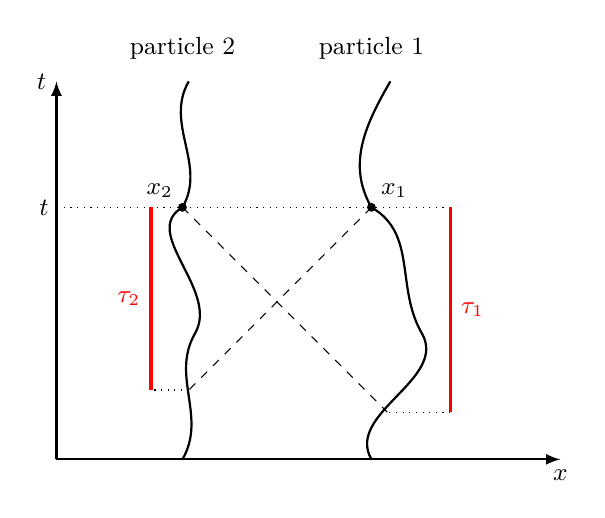
\begin{tikzpicture}[>=latex, every node/.style={font=\small}, scale=0.8]
  % Axes
  \draw[thick, ->](0,0) -- (0,6) node[left] {$t$};
  \draw[thick, ->] (0,0) -- (8,0) node[below] {$x$};

  % Particle 2 worldline (left)
  \coordinate (P2start) at (2,0);
  \coordinate (P2mid)   at (2.2,2);
  \coordinate (P2evt)   at (2,4);
  \coordinate (P2top)   at (2.1,6);
  \draw[thick] (P2start) to[out=60,in=240] (P2mid) 
                to[out=60,in=210] (P2evt) 
                to[out=60,in=240] (P2top);

  % Particle 1 worldline (right)
  \coordinate (P1start) at (5,0);
  \coordinate (P1mid)   at (5.8,2);
  \coordinate (P1evt)   at (5,4);
  \coordinate (P1top)   at (5.3,6);
  \draw[thick] (P1start) to[out=120,in=-60] (P1mid) 
                to[out=120,in=-30] (P1evt) 
                to[out=120,in=-120] (P1top);

  % Events x1 and x2
  \fill (P1evt) circle (2pt) node[above right] {$x_1$};
  \fill (P2evt) circle (2pt) node[above left]  {$x_2$};

  % Dotted equal-time slice
  \draw[dotted] (6.25, 4) -- (0,4);
  \node at (-0.2, 4) {\(t\)};

  \draw[dotted] (6.25, 0.75) -- (5.25,0.75);
  \draw[dotted] (2.1, 1.1) -- (1.5, 1.1);
  

  % Spacelike dashed path
  \draw[dashed] (P1evt) -- (2.1,1.1);
  \draw[dashed] (P2evt) -- (5.25,0.75);


  % Constant-time slices (red)
  \draw[red,very thick] (1.5,1.1) -- (1.5,4)
    node[left,midway] {$\tau_2$};
  \draw[red,very thick] (6.25, 0.75) -- (6.25, 4)
    node[right,midway] {$\tau_1$};

  % Labels for worldlines
  \node at (2,6.2) [above] {particle 2};
  \node at (5,6.2) [above] {particle 1};
\end{tikzpicture}
\end{figure}
    
    \begin{equation}
        F_{12} = F(x_2(t-\tau_2), \dot{x_2}(t-\tau_2), \dots, x_1(t), \dot{x_1}(t), \dots)
    \end{equation}
    and similarly
    \begin{equation}
        F_{21} = F'(x_1(t-\tau_1), \dot{x_1}(t-\tau_1), \dots, x_2(t), \dot{x_2}(t), \dots)
    \end{equation}
    In such an equation, the \(\tau_1\) and \(\tau_2\) themselves are dynamically determined, and depend on the entire past history of the two particles, and therefore in order to determine the dynamics of the particles, one needs to keep track of functions, which have infinite degrees of freedom. \\

    That said, even in classical dynamics, imposing STR postulates demands infinite number of degrees of freedom. 

    \subsection{Quantizing the STR Dynamics}
    In dealing with such systems, we encounter \textit{retarded differential equations}, or also called as \textit{functional differential equations}. And nobody knows how to quantize the system starting from the functional differential equations.\\

    Passage from CM to QM relies strongly on the idea that we are given an initial surface and we have a Hamiltonian/Lagrangian on it.\\
    In a Hamiltonian system we have a phase space and we see how stuff evolves in that space. In the above discussed case, we have to deal with an infinite number of degrees of freedom and these degrees of freedom are not in the form that is convenient to put in the Hamiltonian formalism.\\

    Fields solve this problem by rather than saying that particle 1 interacts with particle 2, we say particle 1 interacts with a field, and particle 2 too interacts with the field. The field and the particles influence each other only locally. In introducing this formalism we paid a price, we introduced infinite number of degrees of freedom in the form of fields, at the effect of removing the necessity of having to track all particle histories. The field can be thought of as keeping track of the history of the particles. In the language of fields, nothing depends on retarded times. \\

    With the introduction of fields, we now have everything in the language of phase space. We are given an initial surface, and data on it, and we can evolve everything into future. But rather than having only finite degrees of freedom we still need to keep track of infinite degrees of freedom of the fields, but they are now in a form convenient to quantize.\\

    \subsection{Another Reason Why We Need Infinite DOFs}
    Heisenberg's uncertainity principle — \(\Delta x \Delta p \ge1 \)\\
    If we have small \(\Delta x\), then \(\Delta p \) becomes large, such that \(\Delta E \ge m\). In this case we are now uncertain if we are dealing with the original particle, or if we have created a new particle. It is convenient therefore, to discuss the particles as excitations of fields, using which one can describe variable number of particles.\\

    ALSO fields explain why all electrons are identical.\\

    \subsection{Regular QM Breaks Causality}
    This is a very generic calculation that can be found in almost all lectures/texbooks. But still included here for completeness. \\

    The regular, single particle quantum mechanics that we all know of and are familiar with breaks causality. Causality requires that a particle can never move faster than the speed of light, i.e.\ a particle initially localised around the position \(\textbf{x}\) should not have any amplitude to move out of the future light cone. Now in the case of single particle QM, consider a particle localised about \(\textbf{x}\), described by state \(\ket{\textbf{x}}\).\\

    Suppose the particle follows the relativistic Hamiltonian, \(\hat H = \sqrt{\hat{\textbf{p}}^2 + m^2}\), the state of the particle after time \(t\) would be \(\exp(-i H t) \ket{\textbf{x}}\). Relativity requires that this state should have zero overlap with \(\ket{\textbf{x}'}\) where \((t, \textbf{x})\) and \((t, \textbf{x}')\) are spacelike separated.\\

    Let \(G(\textbf{x},\textbf{x}') = \braket{\textbf{x}' | \exp(-iHt) \textbf{x}}\). The explicit value of \(G\) can be calculated by inserting the identity in \(\ket{\textbf{p}}\) as follows.

    \begin{equation}
        G(\textbf{x}, \textbf{x}', t) = \int \frac{d^3\textbf{p}}{(2\pi)^3} \braket{\textbf{x}' | \exp(-i\sqrt{\hat{\textbf{p}}^2 + m^2} t) | \textbf{p}} \braket{\textbf{p}|\textbf{x}} = \int \frac{d^3\textbf{p}}{(2\pi)^3} \exp(-i\sqrt{\textbf{p}^2 + m^2} t)\braket{\textbf{x}'| \textbf{p}} \braket{\textbf{p}|\textbf{x}}
    \end{equation}
    \begin{equation}
        G(\textbf{x},\textbf{x}', t) = \int \frac{d^3\textbf{p}}{(2\pi)^3}  \exp(-i\sqrt{\textbf{p}^2 + m^2} t) \exp(-i \textbf{p}\cdot(\textbf{x}-\textbf{x}'))
    \end{equation}
    Write \(\textbf{x} - \textbf{x}' = \textbf{r}\), and align the \(z\) axis to be about \(\textbf{r}\). Then we can convert the above integral into polar coordinates as (where we use \(p = |\textbf{p}|\) and \(r = |\textbf{r}|\))
    \begin{align}
        G(\textbf{r}, t) &= \int \frac{p^2}{(2\pi)^2} \exp(-i\sqrt{p^2 + m^2} t) \exp(-i p r \cos\theta)~ dp d(\cos\theta)\\
        &= \int \frac{p^2}{(2\pi)^2} \exp(-i\sqrt{p^2 + m^2} t) \left( \frac{\exp(-ipr) - \exp(ipr)}{pr} \right)dp\\
        &= \frac{2}{(2\pi)^2}\frac{1}{r}\int \exp(-i\sqrt{p^2 + m^2} t)~ p ~\sin(pr)~dp
    \end{align}
    You can look up this integral in some Russian textbook and find out that this is equal to 
    \begin{equation}
        G \propto K_2 (m\sqrt{r^2 + t^2}) 
    \end{equation}
    This is some finite non-zero number (although it might be small for some values) for all \(r\) and \(t\). Since we require causality to be exactly held, and not approximately held, single particle quantum mechanics breaks causality.

    \newpage
    \section{Classical Field Theory}
    Everything we discussed previously does not logically conclude that the \textit{only} candidates are fields, but fields provide a convenient formalism, and end up solving the problems we were facing. \\

    In general, field is something associated with spacetime. That is, for every spacetime point, it spits out some mathematical entity. For the field, we would like to write a Lagrangian, as an integral of some Lagrangian density over all space. 
    \begin{equation}
        L = \int\ld ~d^3\textbf{x}
    \end{equation}
    We consider Lagrangian densities of the form 
    \begin{equation}
        \ld(\del_\mu \phi(x), \phi(x))
    \end{equation}
    (where we assume the notation \(x = (t, \textbf{x})\)). In principle, the Lagrangian density can be anything, but mostly we consider the most simple forms. We usually start with something that is quadratic in fields and their derivatives. Linear term is ignored since it can be absorbed into the quadratic term by considering a shift by constant factor of the fields leading to the a quadratic Lagrangian.\\
    Example — suppose
    \begin{equation}
        \ld = \frac{1}{2} (\del_\mu \phi)^2 - \frac{1}{2}m^2 \phi^2 - \alpha \phi
    \end{equation}
    consider the transformation \(\phi(x) \to \phi(x) + \displaystyle\frac{\alpha}{m^2}\), with \(\alpha\) being some spacetime independent constant. 
    \begin{equation}
        \ld' = \frac{1}{2} \left( \del_\mu \left(\phi' - \frac{\alpha}{m^2}\right)\right)^2 - \frac{1}{2} m^2 \left(\phi'^2 - 2\frac{\alpha}{m^2} \phi' + \left(\frac{\alpha}{m^2}\right)^2\right) - \alpha \phi = \frac{1}{2} (\del_\mu \phi')^2 - \frac{1}{2}m^2 \phi'^2
    \end{equation}
    (dynamics doesn't change when a constant term is added to the Lagrangian) which is a Lagrangian density with only quadratic terms. 

    \subsection{Dynamics in Classical Field Theory}
    \subsubsection{Lagrangin Dynamics}
    Action — \(S = \int \ld~d^4x\)
    \begin{center}
        \fbox{Nature is lazy}
    \end{center}
    Classical equations of motion — field configurations such that variation of \(S\) under \(\phi \to \phi + \delta\phi\) is zero. \\
    Under such change, 
    \begin{equation*}
        \delta S = \int \frac{\delta \ld}{\delta \del_\mu \phi}\delta(\del_\mu \phi) + \frac{\delta \ld}{\delta \phi}\delta(\phi) ~d^4x
    \end{equation*}
    \begin{equation}
        = \int -\delta\phi \del_\mu\frac{\delta \ld}{\delta \del_\mu \phi} + \delta\phi\frac{\delta \ld}{\delta \phi} + \del_\mu \left( \delta\phi \frac{\delta \ld}{\delta \del_\mu \phi} \right)~d^4x  
    \end{equation}
    Considering variations which vanish at infinity, the last term (which is only a boundary term) vanishes. The other two functions also should vanish for every possible values of \(\delta \phi\), therefore we get the equations of motions to be 
    \begin{equation}
        \del_\mu\frac{\delta \ld}{\delta \del_\mu \phi} - \frac{\delta \ld}{\delta \phi} = 0
    \end{equation}

    \subsubsection{Hamiltonian Dynamics}
    In order to make a passage to QFT, we need a Hamiltonian formulation. In going to Hamiltonian formulation, we trade the \textit{time derivative} with the \textit{conjugate momentum}.\\

    The basic degrees of freedom in classical mechanics were the spatial points \(\textbf{x}\). In the case of the field theory, the basic degrees of freedom are just the fields at a certain instant of time (which we conveniently call \(t=0\)) \(\psi(\textbf{x})\). The \(\del_i \phi(\textbf{x})\) are nothing but linear combinations of the \(\phi(\textbf{x})\), and in going to the Hamiltonian formulation, we treat the time derivative as a different degree of freedom.

    \begin{equation}
        \Pi(t=0, \textbf{x}) = \dot{\phi}(t=0, \textbf{x})
    \end{equation}

    The Hamiltonian is then 
    \begin{equation}
        H(t) = \int \Pi \dot{\phi} - \ld ~d^3\textbf{x} = \int \hd~d^3\textbf{x}
    \end{equation}
    and one can write equations similar to the Hamiltonian equations of motion for the field and its conjugate momenta.

    \subsection{Parameterizing the Phase Space}
    \label{sec:solution-freescalar}
    Given the phase space, the usual parameterization is using \(\Pi\) and \(\Phi\). But we can also parameterize the phase space using different variables — the set of solutions to the equations of motion. This is true because given a point in phase space, we can use it as initial conditions and obtain a solution to the equations of motion. Therefore, there is a one-to-one map between points in phase space and solutions to the equations of motion, and we can see the set of solutions to the equations of motion as parameterizing the phase space. That is, a point corresponds to a solution, and a solution provided a section corresponds to a point.\\
    In other words, the \textit{parameterization} of all solutions to the equations of motion is the same as parameterization of the whole phase space. \\

    For concreteness, let us start considering a specific theory — the scalar free field theory. 
    \begin{equation}
        \ld = \frac{1}{2}\left((\del_\mu \phi)^2 - m^2\phi^2\right)
    \end{equation}
    The equation of motion arising from this lagrangian is simply 
    \begin{equation}
        (\del_\mu \del^\mu + m^2)\phi(x) = (\del_t^2 - \nabla^2 + m^2)\phi(x) = 0
    \end{equation}
    We want to find all possible solutions to this equations of motion in order to parameterize the phase space. To find a parameterization for the solution of the equations of motion, the easiest way is to go to the fourier space. \\
    Writing \(\phi(t, \textbf{x}) = \int d^3\textbf{p} \phi(t, \textbf{p})\exp(i\textbf{p}\cdot\textbf{x})\), we get 
    \begin{equation}
        \int (\del_t^2 + \textbf{p}^2 + m^2)\phi(t, \textbf{p}) d^3\textbf{p} = 0
    \end{equation}
    We are keeping time as it is because in Hamiltonian formulation we require solutions at a given slice of time. \\
    The solutions to the above equation of motion is (with \(\w_\textbf{p} = \sqrt{\textbf{p}^2 + m^2}\))
    \begin{equation}
        \phi(t,\textbf{p}) = a(\textbf{p})\exp(-i \w_\mathbf{p} t) + b(\textbf{p}) \exp(i \w_\mathbf{p} t)
    \end{equation}
    Since we require \(\phi(t, \textbf{x})^* = \phi(t, \textbf{x})\), we need 
    \(\phi(t, \textbf{p})^* = \phi(t, -\textbf{p})\), meaning
    \begin{equation*}
        a^*(\textbf{p})\exp(i \w_\mathbf{p} t) + b^*(\textbf{p}) \exp(-i \w_\mathbf{p} t) = a(-\textbf{p})\exp(-i \w_\mathbf{p} t) + b(-\textbf{p}) \exp(i \w_\mathbf{p} t)
    \end{equation*}
    Comparing, we get \(b(\textbf{p}) = a^*(-\textbf{p})\), therefore, the solutions are 
    \begin{equation}
        \phi(t, \textbf{p}) = a(\textbf{p}) \exp(-i\w_\textbf{p} t) + a^*(-\textbf{p}) \exp(i\w_\textbf{p} t)
    \end{equation}
    and 
    \begin{equation}
        \phi(t, \textbf{x}) = \int a(\textbf{p}) \exp(-i\w_\textbf{p} t + i\textbf{p}\cdot \textbf{x}) + a^*(\textbf{p}) \exp(i\w_\textbf{p} t - i\textbf{p}\cdot \textbf{x}) ~ \frac{1}{\sqrt{2\w_\textbf{p}}} \frac{d^3 \textbf{p}}{(2\pi)^3} 
    \end{equation}
    where in second term, we did the change \(\textbf{p}\to -\textbf{p}\) since the integral is invarient under this change, and \(\displaystyle\frac{1}{\sqrt{2\w_\textbf{p}}}\) is simply a choice of normalisation.\\

    We can also write this as 
    \begin{equation}
        \phi(x) = \int a(p) \exp(-ip.x) + a^*(p) \exp(ip.x) ~\frac{1}{\sqrt{2\w_\textbf{p}}} \frac{d^3 \textbf{p}}{(2\pi)^3} 
    \end{equation}
    where now \(p\) and \(x\) are 4-vectors.\\

    The coordinates on the phase space are \(\phi(t=0, \textbf{x})\) and \(\Pi(t=0, \textbf{x})\), and in this case the parameterization is very clear that 
    \begin{equation}
        \phi(t=0, \textbf{x}) = \int a(\textbf{p}) \exp(i\textbf{p}\cdot \textbf{x}) + a^*(\textbf{p}) \exp(- i\textbf{p}\cdot \textbf{x}) ~ \frac{1}{\sqrt{2\w_\textbf{p}}} \frac{d^3 \textbf{p}}{(2\pi)^3}
    \end{equation}
    and 
    \begin{equation}
        \Pi(t=0, \textbf{x}) = \int -i \left(a(\textbf{p}) \exp(i\textbf{p}\cdot \textbf{x}) - a^*(\textbf{p}) \exp(- i\textbf{p}\cdot \textbf{x}) \right)~ \sqrt{\frac{\w_\textbf{p}}{2}} \frac{d^3 \textbf{p}}{(2\pi)^3}
    \end{equation}
    Rather than parameterizing the phase space using the field and conjugate momentum, we can parameterize using the \(a(\textbf{p})\) and \(a^*(\textbf{p})\). We can also invert these relations to write \(a\) and \(a^*\) in terms of field and momenta.
    \begin{equation}
        a(\textbf{p}) = \sqrt{\frac{\w_\textbf{p}}{2}}\int\phi(0, \textbf{x}) \e^{-i \textbf{p}. \textbf{x}}d^3\textbf{x} + \frac{i}{\sqrt{2\w_\textbf{p}}}\int \Pi(0, \textbf{x})\e^{-i \textbf{p}.\textbf{x}} d^3\textbf{x} 
    \end{equation}
    \begin{equation}
        a^*(\textbf{p}) = \sqrt{\frac{\w_\textbf{p}}{2}}\int\phi(0, \textbf{x}) \e^{i \textbf{p}. \textbf{x}}d^3\textbf{x} - \frac{i}{\sqrt{2\w_\textbf{p}}}\int \Pi(0, \textbf{x})\e^{i \textbf{p}.\textbf{x}} d^3\textbf{x} 
    \end{equation}\\

    \textcolor{red}{
        In order to understand this better, let us do the same analysis for the simpler classical mechanical system of a harmonic oscillator. The equation of motion is 
        \begin{equation*}
            ( \del_t^2 + \w^2 )x = 0
        \end{equation*} This is solved simply by 
        \begin{equation*}
            x(t) = \frac{1}{\sqrt{2\w}}\left(A\exp(-i\w t) + A^*\exp(i\w t)\right) ~~~\because~x\text{ is real}
        \end{equation*}
        where the prefactor is simply a choice of normalisation, and 
        \begin{equation*}
            p(t) = -i\sqrt{\frac{\w}{2}} (A\exp(-i\w t) - A^* \exp(i \w t))
        \end{equation*}
        The coordinates on the phase space are \(x(t=0)\) and \(p(t=0)\), which in this case are 
        \begin{equation*}
            x = \frac{1}{\sqrt{2\w}}(A + A^*)~~\&~~p = -i\sqrt{\frac{\w}{2}} (A - A^*)
        \end{equation*}
        For every \(x, p\), there is a solution \(A\) (where \(A\) is complex) that has \((x,p)\) as its initial conditions, and therefore the set of \(A\) can be thought of as parameterizing the entire phase space. This is exactly what is done in introducing the ladder operators for quantizing the harmonic oscillator. Instead of imposing the quantization condition on the usual coordinates \(x\) and \(p\), one uses the coordinates \(A\) and \(A^*\) and quantizes these degrees of freedom. \\
        Important! — There can be confusion in what one calls a solution to the equation of motion. One might be tempted to assume that, for example in this case, the set of ellipses in the phase space to be the set of solutions to the equations of motions. This is wrong, in the sense that the solutions for motion with initial state \(x_1, p_1\) and with initial state \(x_2, p_2\), even if both lie on the same ellipse, are different. Therefore, given an initial point in phase space, we determine a unique equation that governs this initial point's evolution and this equation is termed a solution. Therefore, corresponding to every point on the phase space, there is a unique solution, and therefore a bijection.  \\      
        }

        \textcolor{red}{
            We can further extend the above discussion by looking at the commutator relations of \(A\) and \(A^*\), which is given by 
            \begin{equation*}
                \{x,p\} = 1 \implies \{A^*, A\} = -i, ~\{A, A\}=0,\{A^*, A^*\} = 0 
            \end{equation*}
            We can also construct the Hamiltonian in terms of the variables \(A\) and \(A^*\), which is given as 
        \begin{equation*}
            H = \frac{1}{2}(p^2 + \w^2x^2) = \frac{1}{2}\w(A^*A+ AA^*) \tag{\(\star\)}
            \label{eq:ham_in_class}
        \end{equation*}
        This reduces to 
        \begin{equation*}
            H = \w A^* A
        \end{equation*}
        The commutators of Hamiltonian with the variables \(A^*\) and \(A\) are 
        \begin{equation*}
            \{H, A^*\} = \w A^*,~~~\{H, A\} = -\w A 
        \end{equation*}
        Notice that all of these are classical calculations, and invokes no quantum mechanics. 
        }
    
    \newpage
    \section{Quantizing the Fields}
    To quantize a theory, we take a set of \textit{coordinates} on phase space, and promote them to operators and impose the commutation relations.\\
    In case of multiple particles in the regular quantum mechanics, the commutation relation that we used to impose was 
    \begin{equation*}
        [x_i, p_j] = i\delta_{ij}
    \end{equation*}
    Similarly, the \(\phi(0, \textbf{x})\) and \(\Pi(0, \textbf{x})\) behave like multiple degrees of freedom, this time instead of labeled by a discrete index \(i\), they are labeled by a continous index \(x\). Therefore, we impose a similar commutation relation
    \begin{equation}
        [\phi(t, \textbf{x}), \Pi(t, \textbf{y})] = i\delta^3(\textbf{x} - \textbf{y})
    \end{equation} 
    \textcolor{red}{
    Notice that these are equal time commutation relations, i.e., this is imposed on one time slice. This is true even in the single particle quantum mechanics, where the canonical commutation relations hold only at equal times, i.e. 
    \begin{equation*}
        [x(t), p(t')] \ne i,~[x(t), x(t')] \ne 0,~[p(t), p(t')]\ne 0
    \end{equation*}
    As an example, consider the harmonic oscillator, 
    \begin{equation*}
        x(t) = \frac{1}{\sqrt{2\w}}(A\exp(-i\w t) + A^*\exp(i\w t))
    \end{equation*}
    \begin{equation*}
        p(t) = -i\frac{\sqrt{\w}}{2}(A\exp(-i\w t) - A^*\exp(i\w t))
    \end{equation*}
    The equal time commutation relation implies 
    \begin{equation*}
        [x(0), p(0)] = i[A, A^*] = i \implies [A, A^*] = 1\text{,~~ and } [A, A] = [A^*,A^*] = 0 
    \end{equation*}
    Using this, 
    \begin{equation*}
        [x(t), x(t')] = \frac{1}{2\w}\left(\e^{i\w(t'-t)}[A, A^*] + \e^{i\w(t-t')}[A^*, A]\right) = \frac{1}{2\w}\cos(\w(t'-t)) \ne 0
        \tag{\(\diamondsuit\)}
        \label{eq:time_comm}
    \end{equation*}
    }

    In terms of \(a(\textbf{p})\) and \(a^\dagger(\textbf{p})\) (where we are now calling \(a^* \equiv a^\dagger\) since we have promoted it to an operator), the commutation relations are 
    \begin{equation*}
        [a(\mathbf{p_1}), a^\dagger(\mathbf{p_2})] = \frac{-i}{2}\int[\phi(0, \mathbf{x_1}), \Pi(0, \mathbf{x_2})]\e^{-i\mathbf{p_1}\cdot \mathbf{x_1}}\e^{i\mathbf{p_2}\cdot \mathbf{x_2}} d^3\mathbf{x_1} d^3\mathbf{x_2} + \frac{i}{2}\int [\Pi(0, \mathbf{x_1}), \phi(0, \mathbf{x_2})]\e^{-i\mathbf{p_1}\cdot \mathbf{x_1}}\e^{i\mathbf{p_2}\cdot \mathbf{x_2}} d^3\mathbf{x_1} d^3\mathbf{x_2}
    \end{equation*}
    \begin{equation}
        = \int \delta^3(\mathbf{x_1} - \mathbf{x_2}) \e^{-i\mathbf{p_1}\cdot \mathbf{x_1}}\e^{i\mathbf{p_2}\cdot \mathbf{x_2}} d^3\mathbf{x_1} d^3\mathbf{x_2} = (2\pi)^2\delta^3(\mathbf{p_1} - \mathbf{p_2})
    \end{equation}
    It also holds that
    \begin{equation}
        [a(\textbf{p}), a(\textbf{q})] = [a^\dagger(\textbf{p}), a^\dagger(\textbf{q})] = 0
    \end{equation}
    \subsection{Hamiltonian in terms of the creation and annihilation operators}
    The expression for Hamiltonian of the theory is 
    \begin{equation}
        H = \frac{1}{2}\int \Pi(0,\textbf{x})^2 + (\nabla \phi(0, \textbf{x}))^2+ m^2\phi(0, \textbf{x})^2 ~d^3\textbf{x}
    \end{equation}
    Calculating this term wise (note that for brevity, we are now calling \(a(\textbf{p}) \equiv a_\textbf{p}\). See that \(a_\textbf{p}\) is not a number, but a function of \(\textbf{p}\)).
    \begin{equation*}
        \frac{1}{2}\int \Pi(0,\textbf{x})^2~d^3\textbf{x} =\frac{1}{2}\int d^3\textbf{x}\frac{d^3\textbf{p}d^3\textbf{q}}{(2\pi)^6}\frac{\sqrt{\w_\textbf{p}\w_\textbf{q}}}{2}\left(-a^\dagger_\textbf{p}a^\dagger_\textbf{q}\e^{i(\textbf{p}+\textbf{q})\cdot \textbf{x}}    
        +a^\dagger_\textbf{p}a_\textbf{q}\e^{i(\textbf{p}-\textbf{q})\cdot \textbf{x}} 
        + a_\textbf{p}a^\dagger_\textbf{q}\e^{-i(\textbf{p}-\textbf{q})\cdot \textbf{x}}   
        - a_\textbf{p}a_\textbf{q}\e^{-i(\textbf{p}+\textbf{q})\cdot \textbf{x}}  
           \right)  
    \end{equation*}
    The integral over \(\textbf{x}\) gives delta functions, and then we can perform an integral over \(\textbf{q}\) to remove the delta function, leading to the simplification
    \begin{equation}
        \frac{1}{2}\int \Pi(0,\textbf{x})^2~d^3\textbf{x} = \frac{1}{2}\int \frac{d^3\textbf{p}}{(2\pi)^3}\frac{\w_\textbf{p}}{2}(-a_\textbf{p}^\dagger a_{-\textbf{p}}^\dagger + a_\textbf{p}^\dagger a_\textbf{p} + a_\textbf{p}a_\textbf{p}^\dagger - a_\textbf{p}a_{-\textbf{p}})
    \end{equation}

    \begin{equation*}
        \frac{1}{2}\int (\nabla \phi(0, \textbf{x}))^2 d^3\textbf{x} = \frac{1}{2} \int d^3\textbf{x}\frac{d^3\textbf{p}d^3\textbf{q}}{(2\pi)^6}\frac{\textbf{p}\cdot \textbf{q}}{2\sqrt{\w_\textbf{p}\w_\textbf{q}}}\left(  
            - a^\dagger_\textbf{p}a^\dagger_\textbf{q}\e^{-i(\textbf{p} + \textbf{q})\cdot \textbf{x}} + a^\dagger_\textbf{p} a_\textbf{q} \e^{i(\textbf{p} - \textbf{q})\cdot \textbf{x}} + a_\textbf{p} a^\dagger_\textbf{q} \e^{-i(\textbf{p} - \textbf{q})\cdot \textbf{x}} - a_\textbf{p} a_\textbf{q} \e^{i(\textbf{p} + \textbf{q})\cdot \textbf{x}}
        \right)
    \end{equation*}
    which again simplifies to 
    \begin{equation}
        \frac{1}{2}\int (\nabla \phi(0, \textbf{x}))^2 d^3\textbf{x} = \frac{1}{2} \int \frac{d^3\textbf{p}}{(2\pi)^3}\frac{\textbf{p}^2}{2\w_\textbf{p}}(a_\textbf{p}^\dagger a_{-\textbf{p}}^\dagger + a_\textbf{p}^\dagger a_\textbf{p} + a_\textbf{p}a_\textbf{p}^\dagger + a_\textbf{p}a_{-\textbf{p}})
    \end{equation}
    and similarly
    \begin{equation}
        \frac{1}{2}\int m^2 \phi(0, \textbf{x})^2 d^3\textbf{x} = \frac{1}{2} \int \frac{d^3\textbf{p}}{(2\pi)^3}\frac{m^2}{2\w_\textbf{p}}(a_\textbf{p}^\dagger a_{-\textbf{p}}^\dagger + a_\textbf{p}^\dagger a_\textbf{p} + a_\textbf{p}a_\textbf{p}^\dagger + a_\textbf{p}a_{-\textbf{p}})
    \end{equation}
    Adding the above three equations, using the fact that \(\w^2_\textbf{p} = \textbf{p}^2 + m^2\), we get 
    \begin{equation}
        H = \frac{1}{2}\int  \frac{d^3\textbf{p}}{(2\pi)^3} \w_\textbf{p} (a_\textbf{p}^\dagger a_\textbf{p} + a_\textbf{p}a_\textbf{p}^\dagger ) 
        \label{eq:hamiltonian}
    \end{equation}

    \subsection{Momentum of Fields}
    Claim — Momentum (not the conjugate momentum, but rather the physical momentum) has the form 
    \begin{equation}
        \textbf{P} = -\int d^3\textbf{x}\Pi(0, \textbf{x}) \mathbf{\nabla} \phi(0, \textbf{x}) 
    \end{equation}
    Why?\\
    We can see that  
    \begin{equation*}
        [\textbf{P}, \phi(0, \textbf{x})] = -i\mathbf{\nabla}\phi(0, \textbf{x})
    \end{equation*}
    Given this commutation relation, we can write, therefore, that 
    \begin{equation}
        \phi(0, \textbf{x} + \mathbf{\epsilon}) = \e^{-i\textbf{P}\cdot\mathbf{\epsilon}}\phi(0, \textbf{x})\e^{i\textbf{P}\cdot\mathbf{\epsilon}} = \phi(0, \textbf{x}) - i[\mathbf{\epsilon}\cdot\textbf{P}, \phi(0, \textbf{x})] = \phi(0, \textbf{x}) + \mathbf{\epsilon}\cdot \mathbf{\nabla}\phi(0, \textbf{x})
    \end{equation}
    Therefore the operator \(\textbf{P}\) generates translations.\\

    In terms of \(a\) and \(a^\dagger\) (the calculation is simple, except that at the end we drop some terms owing to \textit{normal ordering} which will be discussed later) 
    \begin{equation}
        \textbf{P} = \int \frac{d^3\textbf{p}}{(2\pi)^3} \textbf{p}a^\dagger_\textbf{p} a_\textbf{p}
    \end{equation}

    \subsection{Why \(a^\dagger\) and \(a\) are Creation and Annihilation Operators}
    Given the form of Hamiltonian in terms of \(a\) and \(a^\dagger\), we immediately see that 
    \begin{equation}
        [H, a^\dagger_\textbf{p}] = \w_\textbf{p}a^\dagger_\textbf{p},~~~[H, a_\textbf{p}] = -\w_\textbf{p}a_\textbf{p}
    \end{equation}
    which means that for a stationary state \(\ket{E}\) with energy \textbf{E} the operators \(a^\dagger_\textbf{p}\) and \(a_\textbf{p}\) map it to another state with energy \(E+\w_\textbf{p}\) and \(E-\w_\textbf{p}\)
    \begin{equation}
        H(a^\dagger_\textbf{p}\ket{E}) = (E + \omega_p)(a^\dagger_\textbf{p}\ket{E}),~~~ H(a_\textbf{p}\ket{E}) = (E - \omega_p)(a_\textbf{p}\ket{E})
    \end{equation}
    This behavior is exactly the same as that of a harmonic oscillator, and therefore the free Klein-Gordon theory is exactly a decoupled set of infinite harmonic oscillators. 

    \subsection{Constructing the Hilbert Space}
    \subsubsection{Vacuum}
    In order to construct the Hilbert space, we need to start with a vacuum, which is the state with the lowest energy. \\
    Since vacuum has the lowest energy, operating on it with any \(a_\textbf{p}\) should annihilate the state. Therefore, the state vacuum is defined as the state 
    \begin{equation*}
        a_\textbf{p}\ket{0} = 0 ~~\forall \textbf{p}
    \end{equation*}
    The energy of vacuum is 
    \begin{equation*}
        H\ket{0} = \frac{1}{2}\int \frac{d^3\textbf{p}}{(2\pi)^3}\w_\textbf{p} a_\textbf{p} a^\dagger_\textbf{p}\ket{0} =  \frac{1}{2}\int  d^3\textbf{p} \delta^3(0) \w_\textbf{p} \ket{0}
    \end{equation*}
    where we picked the \(\delta(0)\) by commuting the \(a\) and \(a^\dagger\). The result states that the vacuum has infinite energy, which is expected since there are infinite number of harmonic oscillators and each of the oscillator contribute to a finite zero-point energy.\\

    We don't have to worry about this so much because we are able to physically measure only the energy differences, in which case we can set, by-hand, the energy of vacuum to be 0. Another reason why we need not worry is because we are not even sure if the expression for the Hamiltonian is right. This is because when going from classical to quantum theory, there is an inherent ambiuity in operator ordering, and it is upto us to choose what ordering we use. 
    As an example, consider a term \(xp\) in classical physics. How do you write the corresponding operator? There is an ambiguity in whether it will be \(\hat x \hat p\) or \(\hat p \hat x\) or even \(\displaystyle\frac{\hat x \hat p + \hat p \hat x}{2}\) or any other combination. For an example in the case of harmonic oscillator see equation (\ref{eq:ham_in_class}), where the classical variables in the Hamiltonian commute, but there will be an ambiguity in the ordering when promoting the variables to operators. \\

    One convenient choice is to place all the annihilation operator to the right and all the creation operators to the left, and it is called normal ordering, and is denoted as \(\normord{\hat{O}}\). \\

    The normal ordered Hamiltonian is 
    \begin{equation}
        \normord{H} = \int \frac{d^3\textbf{p}}{(2\pi)^3} \w_\textbf{p} a^\dagger_\textbf{p} a_\textbf{p}
    \end{equation}
    and with this choice of \(H\), we get 
    \begin{equation*}
        \normord{H}\ket{0} = 0
    \end{equation*}
    
    \subsubsection{First Excited States} 
    There are an infinite number of first excited states given by 
    \begin{equation*}
        a^\dagger_\textbf{p}\ket{0}
    \end{equation*}
    The energy of these states is \(\w_\textbf{p}\) (since \(\ket{0}\) has energy 0), and momentum
    \begin{equation*}
        \textbf{P}(a^\dagger_\textbf{p}\ket{0}) = \int \frac{d^3\textbf{q}}{(2\pi)^3} \textbf{q}a^\dagger_\textbf{q}a_\textbf{q}a^\dagger_\textbf{p}\ket{0} = \int \frac{d^3\textbf{q}}{(2\pi)^3} \textbf{q}a^\dagger_\textbf{q}(a^\dagger_\textbf{p}a_\textbf{q} + \delta^3(\textbf{p} - \textbf{q}))\ket{0} = \textbf{p}a^\dagger_\textbf{p}\ket{0}
    \end{equation*}
    The energy and momentum indeed satisfy the dispersion relation \(\w_\textbf{p}^2 = \textbf{p}^2 + m^2\), and therefore these are to be interpreted as single particle states. \\

    The normalisation of these states is given as 
    \begin{equation}
        \braket{\textbf{p}|\textbf{q}} = \braket{0|a_\textbf{p}a^\dagger_\textbf{q}|0} = \braket{0|a^\dagger_\textbf{q}a_\textbf{p} + (2\pi)^3\delta^3(\textbf{p}-\textbf{q})|0} = (2\pi)^3\delta^3(\textbf{p}-\textbf{q})
    \end{equation}
    Delta function normalisation does not make any sense physically. Therefore in order to produce a normalisable state, we need to smear the operator, i.e. create a wavepacket
    \begin{equation*}
        \ket{f} = \int f(\textbf{p}) \ket{\textbf{p}} \frac{d^3\textbf{p}}{(2\pi)^3}
    \end{equation*}
    and for this state the normalisation is given by 
    \begin{equation*}
        \braket{f'|f} = \int f'(\textbf{q}) \ket{\textbf{q}} f'(\textbf{p}) \ket{\textbf{p}} \frac{d^3\textbf{p}d^3\textbf{q}}{(2\pi)^6} = \int f'(\textbf{p})f(\textbf{p}) \frac{d^3\textbf{p}}{(2\pi)^3}
    \end{equation*}
    These are not the only states in the Hilbert space of the system, there are other states too.

    \subsubsection{Higher Excited States}
    We can act with multiple creation operators to create higher excited states which can also be interpreted as \(n\)-particle states. As an example, let us check the state \(a^\dagger_\textbf{q}a^\dagger_\textbf{p}\ket{0}\). 
    \begin{equation*}
        H(a^\dagger_\textbf{q}a^\dagger_\textbf{p}\ket{0}) = \w_\textbf{q} + \w_\textbf{p}
    \end{equation*}
    and 
    \begin{align*}
        P(a^\dagger_\textbf{q}a^\dagger_\textbf{p}\ket{0}) &= \int \frac{d^3\textbf{r}}{(2\pi)^3}\textbf{r}a^\dagger_\textbf{r}a_\textbf{r}a^\dagger_\textbf{q}a^\dagger_\textbf{p}\ket{0} \\
        &=\int \frac{d^3\textbf{r}}{(2\pi)^3}\textbf{r}a^\dagger_\textbf{r}( a^\dagger_\textbf{q}a_\textbf{r} +\delta^3(\textbf{q} - \textbf{r}) )a^\dagger_\textbf{p}\ket{0} \\
        &=\int \frac{d^3\textbf{r}}{(2\pi)^3}\textbf{r}a^\dagger_\textbf{r}\delta^3(\textbf{q} - \textbf{r})a^\dagger_\textbf{p}\ket{0}  + \int \frac{d^3\textbf{r}}{(2\pi)^3}\textbf{r}a^\dagger_\textbf{r}a^\dagger_\textbf{q}(a^\dagger_\textbf{p} a_\textbf{r} + \delta^3(\textbf{p} - \textbf{r}))\ket{0} \\
        &= (\textbf{p} + \textbf{q})(a^\dagger_\textbf{q}a^\dagger_\textbf{p}\ket{0} )
    \end{align*}
    Therefore this state has total energy equal to the sum of the energies of one particle states with momentum \(\textbf{p}\) and \(\textbf{q}\), and total momentum equal to the vector sum of the two momenta. Therefore this state can be interpreted as a two particle state with the two particles having the same mass \(m\) and different momenta \(\textbf{p}\) and \(\textbf{q}\).\\

    The two particle states obey bosonic statistics. We can see this by noticing that \(a^\dagger_\textbf{p}\) commutes with \(a^\dagger_\textbf{q}\), and therefore the states \(\braket{\textbf{q}, \textbf{p}}\equiv a^\dagger_\textbf{q}a^\dagger_\textbf{p}\ket{0}\) and \(\braket{\textbf{p}, \textbf{q}} \equiv a^\dagger_\textbf{p}a^\dagger_\textbf{q}\ket{0}\) are the same states. Therefore, these particles automatically satisfy Bose-Einstein statistics, and there is no need to introduce these statistics by hand.\\

    The normalisation of the two particle states can be found as 
    \begin{align*}
        \braket{\mathbf{p_2}, \mathbf{q_2} | \mathbf{p_1}, \mathbf{q_1}} &= \braket{0|\a{p_2}\a{q_2} \adag{p_1}\adag{q_1}|0}\\
        &= \braket{0|\a{p_2} \adag{p_1} \a{q_2} \adag{q_1}|0} + (2\pi)^3\delta^3(\mathbf{q_2} - \mathbf{p_1})\braket{0|\a{p_2}\adag{q_1}|0} \\
        &= \braket{0|\a{p_2} \adag{p_1}|0} (2\pi)^3\delta^3(\mathbf{q_2} - \mathbf{q_1})+ (2\pi)^6\delta^3(\mathbf{q_2} - \mathbf{p_1})\delta^3(\mathbf{p_2} - \mathbf{q_1}) \\
        &= (2\pi)^6\delta^3(\mathbf{q_2} - \mathbf{q_1})\delta^3(\mathbf{p_2} - \mathbf{p_1})+ (2\pi)^6\delta^3(\mathbf{q_2} - \mathbf{p_1})\delta^3(\mathbf{p_2} - \mathbf{q_1}) 
    \end{align*}

    For proper normalisation, we can look at states of the kind 
    \begin{equation*}
        \ket{f} = \int f(\textbf{p}, \textbf{q}) \ket{\textbf{p}, \textbf{q}} \frac{d^3\textbf{p}d^3\textbf{q}}{(2\pi)^6} 
    \end{equation*}
    The smearing function should be symmetric in \(\textbf{p}\) and \(\textbf{q}\), because if there were an antisymmetric part, the bosonic statistics of the state will lead to a zero under the integral.\\
    
    Similarly we can construct \(n\) particle states, with \(n\) going all the way to \(\infty\), by repeated application of creation operators of the respective momenta.\\

    \subsubsection{The Fock Space}    
    With this, we have done all the possible things we could have done on the vacuum, and have generated all the possible states of the theory. Therefore the Hilbert space of the theory is the direct sum 
    \begin{equation}
        \mathbb{H} = \oplus_{n=0}^{\infty}\mathbb{H}_n
    \end{equation}
    where \(\mathbb{H}_n\) is the Hilbert space with \(n\) particles.This is called a Fock Space. In this we are summing over spaces which are orthogonal to each other. \\
    
    \textcolor{red}{
        Check that the one particle states are orthogonal to two particle states.
        \begin{equation*}
            \braket{\textbf{p}, \textbf{q} | \textbf{r}} = \braket{0| \a{p}\a{q}\adag{r}|0} = \braket{0|\a{p}\adag{r}\a{p}|0} + (2\pi)^3\delta^3(\textbf{q} - \textbf{r})\braket{0|\a{p}|0} = 0
        \end{equation*}
        Similarly one can show that the individual spaces are orthogonal to each other.\\
    }

    We can therefore write projectors onto different spaces. 
    \begin{equation*}
        P_0 = \ket{0}\bra{0}
    \end{equation*}
    \begin{equation*}
        P_1 = \int  \frac{d^3\textbf{p}}{(2\pi)^3} \ket{\textbf{p}}\bra{\textbf{p}}
    \end{equation*}
    Why is this a projector? \\
    \begin{equation*}
        P_1^2 = \int  \frac{d^3\textbf{p}d^3\textbf{q}}{(2\pi)^6} \ket{\textbf{p}}\bra{\textbf{p}} \ket{\textbf{q}}\bra{\textbf{q}} = \int  \frac{d^3\textbf{p}}{(2\pi)^3} \ket{\textbf{p}}\bra{\textbf{p}} = P_1
    \end{equation*}
    The projector on 2-particle states is naively
    \begin{equation*}
        P_2 = \int  \frac{d^3\textbf{p}d^3\textbf{q}}{(2\pi)^6} \ket{\textbf{p}, \textbf{q}}\bra{\textbf{p}, \textbf{q}} 
    \end{equation*}
    This is not the complete picture since, 
    \begin{equation*}
        P_2 \ket{\mathbf{k_1}, \mathbf{k_2}} = 2\ket{\mathbf{k_1}, \mathbf{k_2}}
    \end{equation*}
    (use the normalisation derived above, and the fact that the particles are bosons.)\\
    Therefore, we need a prefactor 
    \begin{equation*}
        P_2 = \frac{1}{2!}\int  \frac{d^3\textbf{p}d^3\textbf{q}}{(2\pi)^6} \ket{\textbf{p}, \textbf{q}}\bra{\textbf{p}, \textbf{q}} 
    \end{equation*}
    and therefore, the projector to \(n\)-particle state would be 
    \begin{equation*}
        P_n = \frac{1}{n!}\int  \frac{d^3\mathbf{p_1}\cdots d^3\mathbf{p_n}}{(2\pi)^{3n}} \ket{\mathbf{p_1},\cdots, \mathbf{p_n}}\bra{\mathbf{p_1},\cdots, \mathbf{p_n}} 
    \end{equation*}

    The identity therefore would be 
    \begin{equation*}
        \mathbb{I} = \sum_{i=0}^\infty P_i
    \end{equation*}
    
    \newpage
    \section{Detour — Schrodinger Representation}
    So far we discussed \textit{one} representation of the Hilbert Space. Here we will discuss another representation called the Schrodinger representation. (Hattfeld — QFT of particles and strings, and Polchinski — String theory).

    \subsection{The Schrodinger Equation}

    Initially we told that field theory is not different from QM, but so far we have not discussed any wavefunctions or Schrodinger equation governing the evolution of the wavefunction. It is indeed possible to do so, just that it is not a convenient picture to speak about the fields in terms of. Here we discuss the picture a bit.\\

    We started our quantization procedure through the commutation relations
    \begin{equation}
        [\phi(0, \textbf{x}), \Pi(0, \textbf{x}')] = i\delta^3(\textbf{x} - \textbf{x}')
    \end{equation}
    There is also a natural way to also represent states, which is to think of wavefunctions on the different degrees of freedom, i.e. in this case it will become a wavefunctional 
    \begin{equation}
        \psi[\phi(0,\textbf{x})]
    \end{equation}
    In normal QM, if you give a value of \(\textbf{x}\) at an instant of time, it spits out a c-number. In the case of QFT, when you give a field configuration in space at an instant of time, the wavefunctional gives a c-number. \\

    An example of such a wavefunction is 
    \begin{equation}
        \psi[\phi] = \e^{-\int \phi(0, \textbf{x})^2d^3\textbf{x}}
    \end{equation}
    The constraint on the possible functionals is that it should be normalisable.\\

    How does the momentum acts on the wavefunction?\\
    Claim — The momentum operator is given by the following operator on the wavefunction 
    \begin{equation}
        \Pi(0, \textbf{x}) = -i\frac{\delta}{\delta\phi(0, \textbf{x})}
    \end{equation}
    To check that this is indeed the form of momentum operator, check
    \begin{align*}
        [\phi(0, \textbf{x}), \Pi(0, \textbf{y})]\psi &= -i\left( \phi(0, \textbf{x}) \frac{\delta}{\delta \phi(0, \textbf{y})} \psi - \frac{\delta}{\delta \phi(0, \textbf{y})}(\phi(0, \textbf{x}) \psi)  \right)\\
        &=i \delta^3(\textbf{x} - \textbf{y})\psi       
    \end{align*}
    as required.\\

    \textcolor{red}{
        We can also check that the momentum operator acts as translation operator on the wavefunctional when we perform a shift on the field configuration. An infinitesimal shift in the field configuration is of the form 
        \begin{equation}
            \phi(0, \textbf{x}) \to \phi(0, \textbf{x}) + \epsilon \varphi(0, \textbf{x})
        \end{equation}
        Under such a transformation, the wavefunctional transforms as 
        \begin{equation}
            \psi[\phi(0, \textbf{x}) + \epsilon \varphi(0, \textbf{x})] \approx \psi[\phi(0, \textbf{x})] + \epsilon \varphi(0, \textbf{x})\frac{\delta }{\delta  \phi(0, \textbf{x})}\psi[\phi(0, \textbf{x})] = \e^{i\epsilon\varphi(0, \textbf{x}) \left( -i\frac{\delta}{\delta \phi(0, \textbf{x})} \right)}\psi[\phi(0, \textbf{x})]
        \end{equation}
        If we require momentum operator to generate these translations, then the momentum operator must be indeed of the form 
        \begin{equation}
            \Pi(0, \textbf{x}) = -i\frac{\delta}{\delta \phi(0, \textbf{x})}
        \end{equation}
        Therefore, the theory has three momentums which one can talk about — the conjugate momentum to \(\textbf{x}\) - \(\textbf{p}\) which generates translations in space, the physical momentum operator \(\textbf{P}\) which generates translations of fields in space, i.e. \(\phi(0, \textbf{x}) \to \phi(0, \textbf{x} + \textbf{a})\), and has as eigenvalues the total momentum of the excitations, and the momentum conjugate to the fields, \(\Pi\) which generates the translations of wavefunctional under shifts in field configurations, i.e. \(\psi[\phi] \to \psi[\phi + \varphi]\).\\
        In a similar language as QM, we can also write wavefunctions in other spaces such as momentum space in configuration space, by making a fourier transformation of \(\psi[\phi]\) with respect to \(\Pi\) and converting to \(\psi[\Pi]\) given as 
        \begin{equation}
            \psi[\Pi] = \int \D \phi ~\psi[\phi] \e^{-i\int \phi \Pi d^3\textbf{x}}
        \end{equation}
        but at this point, such a fourier transform has no use to it in our disccussions.\\
    }

    We can also write a Schrodinger equation given as 

    \begin{equation}
        i\frac{\del}{\del t}\psi[\phi] = \int -\frac{\delta^2}{\delta \phi^2} \psi[\phi] + (\nabla \phi)^2\psi[\phi]+ m^2\phi^2\psi[\phi]  ~~d^3\textbf{x}
    \end{equation}
    which governs the time evolution of the wavefunctional.

    \subsection{The Vacuum in Schrodinger Formulation}
    The defining property of vacuum is that the annihilation operators annihilate the vacuum. 
    It is convenient to introduce the fourier transform 
    \begin{equation}
        \phi(0, \textbf{p}) = \int \phi(0, \textbf{x}) \e^{-i\textbf{p}\cdot \textbf{x}}d^3\textbf{x}
    \end{equation}
    \begin{equation}
        \Pi(0, \textbf{p}) = \int \Pi(0, \textbf{x}) \e^{-i\textbf{p}\cdot \textbf{x}}d^3\textbf{x}
    \end{equation}
    In terms of these, the commutation relation is 
    \begin{equation}
        [\phi(0, \textbf{p}), \Pi(0, \textbf{q})] = \int [\phi(0, \textbf{x}), \Pi(0, \textbf{y})]\e^{-i\textbf{p}\cdot\textbf{x}}\e^{-i\textbf{q}\cdot \textbf{y}} d^3\textbf{x}d^3\textbf{y} = i(2\pi)^3\delta^3(\textbf{p}+\textbf{q})
    \end{equation}
    The action of \(\Pi(0, \textbf{p})\) on \(\psi\) is given by 
    \begin{equation}
        \Pi(0, \textbf{p})\psi[\phi(0, \textbf{q})] = -i(2\pi)^3\frac{\delta}{\delta \phi(0, -\textbf{p})}\psi[\phi(0, \textbf{q})]
    \end{equation}

    \textcolor{red}{
        To check that this is true, see that
        \begin{equation}
            [\psi(0, \textbf{p}), \Pi(0, \textbf{q})]\psi = -i(2\pi)^3 \left( \phi(0, \textbf{p}) \frac{\delta}{\delta \phi(0,-\textbf{q})}\psi - \frac{\delta}{\delta(\phi(0, -\textbf{q}))} (\phi(0, \textbf{p})\psi)\right) = i(2\pi)^3\delta^3(\textbf{p}-~(-\textbf{q}))
        \end{equation}
        which is indeed the required relation.\\
    }

    We had 
    \begin{equation}
        a_\textbf{p} = \sqrt{\frac{\w_\textbf{p}}{2}}\int\phi(0, \textbf{x}) \e^{-i \textbf{p}. \textbf{x}}d^3\textbf{x} + \frac{i}{\sqrt{2\w_\textbf{p}}}\int \Pi(0, \textbf{x})\e^{-i \textbf{p}.\textbf{x}} d^3\textbf{x} 
    \end{equation}
    which now becomes 
    \begin{equation}
        a_\textbf{p} = \sqrt{\frac{\w_\textbf{p}}{2}}\phi(0, \textbf{p}) + \frac{i}{\sqrt{2\w_\textbf{p}}}\Pi(0,\textbf{p})
    \end{equation}
    The vacuum is the state that is annihilated by \(a_\textbf{p}\) which gives the equation
    \begin{equation}
        \sqrt{\frac{\w_\textbf{p}}{2}}\phi(0, \textbf{p}) \psi_0[\phi] -i(2\pi)^3 \frac{i}{\sqrt{2\w_\textbf{p}}}\frac{\delta}{\delta \phi(0, -\textbf{p})}\psi_0[\phi] = 0
    \end{equation}
    This is solved by 
    \begin{equation}
        \psi_0 = \displaystyle\e^{-\frac{1}{2}\int \w_\textbf{p} \phi(0, \textbf{p})\phi(0, -\textbf{p})\frac{d^3\textbf{p}}{(2\pi)^3}}
    \end{equation}
    Since \(\phi(0, \textbf{x})\) is real field, we need that \(\psi(0, -\textbf{p}) = \psi(0, \textbf{p})^*\). Therefore the solution is an exponential of squares, which means it is a Gaussian, as was in the case of harmonic oscillator. Notice that this ground state is not normalised. In such a formalism, the expectation values are to be written as 
    \begin{equation}
        \braket{A} = \displaystyle \frac{\int \D \phi ~ \psi[\phi]^2 A[\phi] }{\int \D \phi ~ \psi[\phi]^2}
    \end{equation}
    and therefore the normalisation doesn't matter as it gets cancelled when taking the ratios.\\

    Similarly we can also write the wavefunctionals for higher excited states by acting upon with \(a^\dagger_\textbf{p}\)s.

    \newpage
    \section{Causality}
    Before discussing causality, we need a notion of what are the observables in a QFT. 

    \subsection{Observables in QFT}
    In quantum mechanics all Hermitian operators are observables. When transitioning to QFT, we need to modify our notion of the observables. In QFT, observables are tied to spacetime points.\\

    Observables are of the form \(O(x)\) (where \(x\) is now a spacetime point). We can define observables in a region \(R\) as 
    \begin{equation}
        \int_R O(x) f(x) d^4x
    \end{equation}
    We can also construct operator like 
    \begin{equation}
        \int_{\bar{R}} O(x) g(x) d^4x
    \end{equation}
    where \(\bar{R}\) is the region complement to \(R\), and this operator is NOT an observable in \(R\).\\

    \subsection{Does QFT Preserve Causality}

    Suppose \(R\) and \(R'\) are spacelike separated regions. Then causality requires that observations in \(R\) should be independent of observations in \(R'\). What this means is that observations in \(R\) should not affect, and should not be affected by observations in \(R'\). What this implies is that 
    \begin{equation}
        [O(R) , \tilde O(R')] = 0
    \end{equation}
    This doesn't mean that observation in \(R\) should be uncorrelated with observations in \(R'\). They can be correlated as in entanglement, but they should not be able to affect each other. Notice that we have always used this notion in our regular quantum mechanics, where we say that when measuring one observable does not affect the value of another should imply that they have a simultaneous set of eigenvalues and therefore the operators must commute. Here we are running a similar argument. \\

    All observables in our theory are polynomials in \(\phi\). Therefore causality requires that 
    \begin{equation}
        [\phi(x), \phi(y)] = 0\text{, if }(x-y)^2 <0
    \end{equation}
    On a single time slice, this is true and is a canonical commutation relation, since every \(\textbf{y}\) is disconnected from \(\textbf{x}\). But causality requires this to be true also for any \(x\) and \(y\) at different times, but spacelike separated. (The commutator relation above being satisfied at \(t=0\) doesn't guarentee that it will be satisfied at some other \(t\) as can be seen in the example (\ref{eq:time_comm}))\\

    Is this criteria satisfied in our theory?\\
    We can explicitly calculate this commutator as follows 
    \begin{equation*}
        \phi(x) = \int \a{p}\e^{-ip\cdot x} + \adag{p}\e^{ip\cdot x} \frac{d^3\textbf{p}}{(2\pi)^3\sqrt{2\w_\textbf{p}}}
    \end{equation*}
    \begin{equation*}
        \implies [\phi(x), \phi(y)] = \int [\a{p}, \adag{q}]\e^{-ip\cdot x + iq\cdot y} + [\adag{q}, \a{p}]\e^{ip\cdot x - iq\cdot y}\frac{d^3\textbf{p}d^3\textbf{q}}{(2\pi)^62\sqrt{\w_\textbf{p}\w_\textbf{q}}}
    \end{equation*}
    \begin{equation*}
        = \int \e^{-ip\cdot(x-y)} - \e^{ip\cdot(x-y)}\frac{d^3\textbf{p}}{(2\pi)^32\w_\textbf{p}}~~
    \end{equation*}
    The LHS is Lorentz invarient, but on RHS, we see that the integral is over \(d^3\textbf{p}\). The RHS should still be Lorentz invarient. To see how we can write the integral in a covariant form, consider the following integral first
    \begin{equation}
        \int d^4p \delta^4(p^2 - m^2) \theta(p^0)
    \end{equation}
    Now this integral is manifestly Lorentz invarient, because it has an integral over \(d^4p\), a \(\delta\) function in \(p^2 - m^2\) and a \(\theta\) function in \(p^0\). The \(\theta\) function is also Lorentz invarent since \(\delta\) function fixes that \(p^2 = m^2 >0\), making \(p\) a timelike vector, and there is no Lorentz transformation that can change the sign of the time component of a timelike vector. The \(theta\) function is also needed since we initially started with a specific sign of \(\w\), that is \(\w_p >0\). If we choose the other sign, then the result will not be that of the integral we are trying to evaluate.\\
    We can do this integral as 
    \begin{align*}
        &\int d^3\textbf{p}dp^0 \delta(p_0^2 - \textbf{p}^2 - m^2)\delta(p^0)\\
        =& \int d^\textbf{p}dp^0 \frac{\delta(p_0 - \w_p)}{2p_0}\\
        =& \int \frac{d^3\textbf{p}}{2\w_p}
    \end{align*}
    Therefore, the commutator can be written as a Lorentz invarient integral 
    \begin{equation}
        [\phi(x), \phi(y)] = \int \e^{-ip\cdot(x-y)} - \e^{ip\cdot(x-y)}\frac{1}{(2\pi)^3}d^4p \delta^4(p^2 - m^2) \theta(p^0)
    \end{equation}
    When \(x\) and \(y\) are spacelike separated, there is a Lorentz transformation that takes \(x-y\) to \(-(x-y)\). An explicit example would be to first boost to a frame where \(x\) and \(y\) are simultaenous, making \(x-y = (0, \mathbf{\Delta})\), and then a rotation of the \(3-\)vector by 180 degree taking it to \((0.-\mathbf{\Delta}) = -(x-y)\). Notice that this is not possible when \(x\) and \(y\) are timelike separated, since there is no frame of reference where they are simultaneous. Therefore, when \(x\) and \(y\) are timelike separated, the second integral can be Lorentz transformed to match the first integral, and therefore the difference between them, which gives the commutator, is zero.\\

    We also need to check that the commutator is not identically zero when the separation is timelike. To check this, we need to explicitly evaluate the integral by converting it into polar coordinates.  \\
    Consider the integral 
    \begin{align*}
        f(q) &= \int e^{-ip\cdot q} \frac{d^3\textbf{p}}{(2\pi)^3{2\w_\textbf{p}}} = \e^{-i\w_p q^0} \int \e^{i\textbf{p}\cdot \textbf{q}} \frac{d^3\textbf{p}}{(2\pi)^3{2\w_\textbf{p}}}\\
        &= \e^{-i\w_p q^0} \int \e^{ipq\cos\theta} p^2 dp d\cos\theta\frac{1}{(2\pi)^2{2\w_\textbf{p}}} \text{where now }p~\&~q\text{ stand for } |\textbf{p}|~\&~|\textbf{q}|\\
        &= \e^{-i\w_p q^0}\int_0^\infty \frac{1}{iq}\left(  \e^{ipq} - \e^{-ipq}  \right) pdp \frac{1}{(2\pi)^2{2\w_\textbf{p}}}
    \end{align*}
    Since the integral is invarient under the transformation \(p\to-p\), we can do the transformation for the second piece, and then flip the integration limits, to obtain 
    \begin{align*}
        f(q) &= \e^{-i\w_p q^0}\int_0^\infty \frac{1}{iq} \e^{ipq} pdp \frac{1}{(2\pi)^2{2\w_\textbf{p}}} + \e^{-i\w_p q^0}\int_{-\infty}^0 \frac{1}{iq} \e^{ipq} pdp \frac{1}{(2\pi)^2{2\w_\textbf{p}}}\\
        &=\e^{-i\w_p q^0}\int_{-\infty}^\infty \frac{1}{iq} \e^{ipq} pdp \frac{1}{(2\pi)^2{2\w_\textbf{p}}}\\
        &= \frac{-i}{4\pi q} \frac{\del}{\del q} \int_{-\infty}^{\infty} \e^{-i\w_p q^0+ipq} \frac{dp}{2\pi\w_p} 
    \end{align*}
    Now, we can make the substitutions 
    \begin{align*}
        \w_p = m\cosh\phi ~~&\&~~ p = m\sinh \phi \implies \frac{dp}{\w_p} = d\phi\\
        q^0 = \alpha \cosh\phi_0 ~~&\&~~ q = \alpha\sinh \phi_0 
    \end{align*}
    This substitution also preserves the relations between \(\w_p\) \& \(p\) and \(q^0\) \& \(q\). Also we are taking \(q^0\) with \(\cosh\) because we are looking at the case where \(q^0\) is large compared to \(q\).\\

    With this, we can write the integral as 
    \begin{equation*}
        f(q) = \frac{-i}{4\pi q} \frac{\del}{\del q} \int_{-\infty}^\infty \e^{-im\alpha \cosh(\phi -\phi_0)} \frac{d\phi}{2\pi} 
    \end{equation*}
    This integral has the value 
    \begin{equation*}
        f(q) = \frac{1}{4\pi} \frac{\del}{\del q} \left(-\frac{i}{2} \mathrm{sgn}(q^0) J_0(m\alpha) - N_0(m\alpha)\right)
    \end{equation*}
    (there seems to be some errors in the calculation. If you are able to rectify please send your calculations by email!)\\
    The commutator in the case \(x-y\) is timelike is therefore 
    \begin{equation*}
        [\phi(x), \phi(y)] = \frac{i}{4\pi} \mathrm{sgn}(x^0 - y^0) \frac{m}{\alpha} J_1(m\alpha)
    \end{equation*}
    We get this as, differentiation of \(J_0\) gives \(J_1\) and when taking the Hermitian conjugate of the above integral and subtracting it to get the commutator, the term proportional to \(N_1\) cancels. It should not be surprising that the answer is proportional to \(i\) since the commutator is an antihermitian quantity and therefore should be purely imaginary. \\

    The commutator is finite in timelike separations and exactly zero for spacelike separations. \\
    Therefore, causality is preserved in QFT.
    
    \subsection{Localized Excitations in QFT}
    \textcolor{red}{Before discussing localised excitations, let us first discuss what the action of \(\phi(x)\) on the vacuum is. We called \(\adag{p}\ket{0}\)s as the one particle states of our system. The \(\phi(x)\) is a linear combination of \(\adag{p}\)s, with different \(p\)s given different weights. Therefore, \(\phi(x)\ket{0}\) is a superposition of infinite number of one particle states with different momenta, and therefore is itself a one particle state. To create higher particle states, one needs to operate by more \(\phi(x)\)s \\}

    Now let us discuss how can one define localised excitations in some region \(R\)?\\
    Suppose we have a region \(R\), and an operator \(O\) in \(\bar{R}\) which is spacelike to \(R\)
    \begin{figure}[h]
        \centering 
        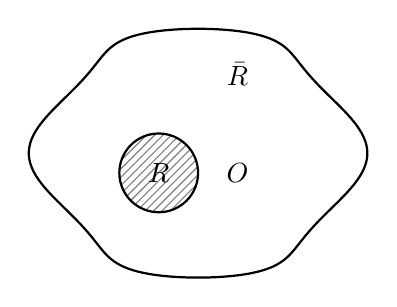
\begin{tikzpicture}
            \draw[thick]
                plot [domain=0:360, samples=200, smooth, variable=\t]
                    (
                        {0.5 + 2*cos(\t) + 0.15*cos(5*\t)},
                        {0.25 + 1.5*sin(\t) + 0.08*sin(1*\t)}
                    )
                    -- cycle;
            \fill[pattern=north east lines, pattern color=black!50] (0,0) circle (0.5);
            \draw[thick] (0,0) circle (0.5);
            \node at (0,0) {\(R\)};
            \node at (1,1.25) {\(\bar R\)};
            \node at (1, 0) {\(O\)};
        \end{tikzpicture}
    \end{figure}

    For an excitation \(\ket{\psi(R)}\) to be local in \(R\), we require that 
    \begin{equation*}
        \braket{\psi(R)|O(\bar{R}) | \psi(R)} = \braket{0|O(\bar{R})|0} ~~\forall~O \text{ in region spacelike to }R
    \end{equation*} 
    That is, the expectation values of operators in regions spacelike separated from \(R\) should be the same as their vacuum expectation values.  \\

    How can we create such a state?\\
    Our first guess would be 
    \begin{equation*}
        \ket{\psi(R)} = \int_R d^4x f(x) \phi(x) \ket{0} 
    \end{equation*}
    We can check if this is indeed a localised expectation, 
    \begin{equation*}
        \braket{\psi(R)|O(\bar{R})|\psi(R)} = \int f(x) f(y) \braket{0|\phi(x) O \phi(y) | 0}
    \end{equation*}
    since \(\phi\) in \(R\) and \(O\) in \(\bar{R}\) must commute, the above should be equal to 
    \begin{equation*}
        \braket{\psi(R)|O(\bar{R})|\psi(R)} = \int f(x) f(y) \braket{0|O\phi(x)  \phi(y) | 0}
    \end{equation*}
    which is not equal to the vacuum expectation value of \(O\). See that even \(\phi(z)\) does not produce a local excitation \textbf{at \(z\)}, since \(\phi(z)\) is obtained by simply setting \(f(x) = \delta(x-z), ~f(y) = \delta(z-y)\) in the above integral.  \\

    What do we need to create a localized excitation?\\
    In order for \(\ket{\psi(R)} = U(R)\ket{0}\) to be a localised excitation, we need 
    \begin{equation*}
        \braket{\psi(R)|O(\bar{R})|\psi(R)} = \braket{0|U^\dagger(R)O(\bar{R})U(R)|0} = \braket{0|O(\bar{R})U^\dagger(R)U(R)|0} = \braket{0|O(\bar{R})|0}
    \end{equation*}
    What this implies is that the operator \(U\) should satisfy \(U^\dagger U = I\), i.e.\ it should be unitary. Therefore 
    \begin{equation*}
        U(R) = \e^{i\int_R f(x)\phi(x) dx}\ket{0}
    \end{equation*}
    is a localised excitation in \(R\). There is no unique localised excitation, there can be many unitary operators in \(R\) that can produce localised excitations. One can also see that since \(\phi\) are Hermitian, the only way to create unitary operators is by exponentiating the \(\phi\)s with a factor of \(i\). If you produce an excitation in a region of space \(\textbf{R}\), it propagates outwards at the speed of light, such that all the region which is timelike to \(\textbf{R}\) is affected, while regions spacelike to \(\textbf{R}\) are not at all affected. \\
    
    Now these localised excitations can never be single particle states. Since the exponential can be written as 
    \begin{equation*}
        \e^{i\int_R f(x)\phi(x) dx}\ket{0} = \left(1 + i\int_R f(x)\phi(x) dx + \frac{1}{2}i\iint_R f(x)f(y)\phi(x)\phi(y) dxdy + \cdots \right)\ket{0}
    \end{equation*}
    the localised excitation is always a superposition of states of all possible particle numbers. 

    \newpage
    \section{Interlude — Symmetries}

    What we mean when we say that the action has symmetry is that when we make a change in the fields \(\phi_i(x) \to \phi_i(x) + \lambda D\phi_i(x)\), (where \(D\phi_i\) is just a notation and can denote any function, but is usually a function of original \(\phi_i\)s and \(\lambda\) is a parameter to keep track of order of terms), the action remains invariant. \\
    For this to be true, the Lagrangian density should transform as 
    \begin{equation*}
        \ld \to \ld + \del_\mu K^\mu
    \end{equation*}
    Now this invariance should hold for all the field configurations, and not just some special ones, i.e.\ the configurations which satisfy the equations of motion. For the configurations which satisfy the equations of motion, the requirement is identically satisfied, since we define the equations of motion as those configurations for which the small variations of fields do not change the action.\\ 

    \subsection{Noether's Theorem}
    When \(\ld\) has a symmetry, there is a conserved current of the form
    \begin{equation*}
        \del_\mu j^\mu = 0
    \end{equation*} 
    \textit{only for the solutions of the equations of motion}.\\

    Proof —\\
    Under the above transformation,
    \begin{align*}
        &\delta \ld = \left( \frac{\delta \ld}{\delta \phi_i} D\phi_i  + \frac{\delta \ld}{\delta \del_\mu \phi_i} \del_\mu D\phi_i \right) = \del_\mu K^\mu \\
        \implies & \left( \frac{\delta \ld}{\delta \phi_i} D\phi_i  -\del_\mu \frac{\delta \ld}{\delta \del_\mu \phi_i} D\phi_i + \del_\mu \left( \frac{\delta \ld}{\delta \del_\mu \phi_i} D\phi_i \right)  \right) = \del_\mu K^\mu 
    \end{align*}
    When we are on-shell (i.e. when \(\phi\) satisfies the equation of motion), the first two term sum to 0, and we are left with 
    \begin{equation*}
        \del_\mu \left( \frac{\delta \ld}{\delta \del_\mu \phi_i} D\phi_i \right) = \del_\mu K^\mu
    \end{equation*}
    which implies that  
    \begin{equation*}
        \del_\mu j^\mu(x) =0, ~\text{ where  } j^\mu = \frac{\delta \ld}{\delta \del_\mu \phi_i} D\phi_i  - K^\mu 
    \end{equation*}

    Noether's current is not something new, it is just re-expressing the equations of motion. Noether's current has inherent ambiguity in definition, because we can always add a divergence free \(4-\)vector to it, i.e.\ we can add terms of the form \(\epsilon^{\mu\nu} \del_\nu \phi\) where \(\epsilon\) is antisymmetric tensor, since \(\del_\mu \epsilon^{\mu\nu} \del_\nu \phi = 0\). But nevertheless this is a powerful statement and allows us to derive conclusions without having to do tedious calculations.\\

    When we have a conserved current, we have a conserved charge.
    \begin{equation*}
        \del_0 \int j^0 d^3\textbf{x} + \int d^3\textbf{x} \del_i j^i = 0 \implies \del_t \int j^0 d^3\textbf{x} = 0
    \end{equation*}
    since the second term is a total divergence. What this tells is that the quantity 
    \begin{equation*}
        Q = \int j^0 d^3\textbf{x}
    \end{equation*} 
    is conserved. All conservation of laws that we have known so far arise in this very fashion, and are consequences of the Noether's theorem.\\

    There is another derivation of the Noether's theorem, which is at the level of action. Suppose we have a symmetry under 
    \begin{equation*}
        \phi \to \phi + \lambda D\phi
    \end{equation*}
    which does not change \(S\).\\
    Now imagine a spacetime dependent variation, 
    \begin{equation*}
        \phi \to \phi + \lambda(x) D\phi
    \end{equation*}
    The action is not invarient under this transformation. The Lagrangian, upto first order in \(\lambda\) changes as 
    \begin{equation*}
        \ld \to \ld + \lambda(x) \del_\mu(K^\mu) + \del_\mu(\lambda(x)) P^\mu
    \end{equation*}
    since these are the only terms that are Lorentz invariant and first order in \(\lambda\).\\
    The action transforms as 
    \begin{align*}
        S \to &S + \int d^4x~ \lambda(x) \del_\mu(K^\mu) + \del_\mu(\lambda(x)) P^\mu\\
        = & S + \int d^4x ~ \lambda(x) \del_\mu (K^\mu - P^\mu)
    \end{align*}
    On solutions to equations of motions, the action should be invariant under these transformations too. Therefore 
    \begin{equation*}
        \del_\mu (K^\mu - P^\mu) = 0
    \end{equation*}
    Now what is \(P^\mu\)? \\
    Under the given transformation, the Lagrangian changes as 
    \begin{equation*}
        \ld \to \ld + \left( \frac{\delta \ld}{\delta \phi}\lambda(X) D\phi +  \frac{\delta \ld}{\delta \del_\mu \phi} \del_\mu(\lambda(x) D\phi) \right)
    \end{equation*}
    from which we can see that \(P^\mu\) is simply the part that multiplies to \(\del_\mu \lambda(x)\), which is 
    \begin{equation*}
        P^\mu = \frac{\delta \ld}{\delta \del_\mu \phi} D\phi
    \end{equation*}

    % We can also ask how the conserved charge transform under Lorentz transformation.\\

    % The conserved current is a \(4-\)vector, and therefore under Lorentz transformation transforms as
    % \begin{equation*}
    %     J^\mu(x) \to J'^{\mu}(x') = \Lambda\indices{^\mu_\nu}J^\nu (\Lambda^{-1} X)
    % \end{equation*}
    % The conserved charge is given by 
    % \begin{equation*}
    %     Q(t) = \int d^3\textbf{x} J^0(t, \textbf{x})
    % \end{equation*}
    % Now since this is conserved, we can choose one specific time to evaluate this, and for convenience we choose \(t=0\).\\
    % \begin{equation*}
    %     Q = \int d^3\textbf{x} J^0(0, \textbf{x})
    % \end{equation*}
    % We can also write this as the \(4-\)integral
    % \begin{equation*}
    %     Q = \int d^4x \delta(\eta\cdot x) \eta \cdot J(x)
    % \end{equation*}
    % where \(\eta = (1,0,0,0)\). This \(4-\)integral can be written as 
    % \begin{equation*}
    %     Q = \int d^4x \del_\mu \theta(\eta\cdot x)  J^\mu(x)
    % \end{equation*}
    % by noticing that the space-derivative of theta function is simply zero, and the time derivative gives the delta function multiplied by \(\eta_\mu\)
    

    \subsection{Applications}
    Let us look at some applications of the Noether's theorem
    \subsubsection{Spacetime translations}
    Consider \(x^\mu \to x^\mu + a^\mu\).\\
    When \(\ld\) doesn't explicitly depend on position, this is a symmetry. In the language of fields, this transformation is 
    \begin{equation*}
        \phi \to \phi + \lambda \del_\mu \phi^\mu 
    \end{equation*}
    where \(\lambda\) is just to keep track of orders.\\

    Since \(\ld\) is a Lorentz scalar, 
    \begin{equation*}
        \ld \to \ld + \lambda a^\mu \del_\mu \ld \implies K^\mu =  a^\mu \ld
    \end{equation*}

    Therefore, the conserved current is 
    \begin{equation*}
        j^\mu = \frac{\delta \ld}{\delta \del_\mu \phi}a^\nu  \del_\nu \phi  - a^\nu \delta_\nu^\mu \ld
    \end{equation*}
    Now this current is conserved for all possible \(a^\mu\) which means that 
    \begin{equation*}
        T_\nu^\mu = \frac{\delta \ld}{\delta \del_\mu \phi} \del_\nu \phi  -  \delta_\nu^\mu \ld \implies T^{\mu\nu} = \frac{\delta \ld}{\delta \del_\mu \phi} \del^\nu \phi  -  \eta^{\mu\nu} \ld
    \end{equation*}
    must be conserved. This is called stress-energy tensor and this is conserved. Let us check what this is for few cases 
    \begin{equation*}
        T^{00} = \frac{\delta \ld}{\delta \dot{\phi}}  \dot{\phi} - \ld = \mathcal{H}
    \end{equation*}
    which is the Hamiltonian density. Integrating this over all space gives the Hamiltonian which is the energy, and this shows that energy is conserved.
    \begin{equation*}
        T^{0i} = \frac{\delta \ld}{\delta \dot{\phi}} \del^i \phi
    \end{equation*}
    the corresponding conserved charge is 
    \begin{equation*}
        P^i =  \int d^3\textbf{x} \frac{\delta \ld}{\delta \dot{\phi}} \del^i \phi
    \end{equation*}
    which is nothing but the spatial momentum in \(i\)th direction as we had defined previously. The stress tensor therefore gives \(4\) conserved charges (we need to keep \(\mu = 0\) and integrate, and there are \(4\) choice of \(\nu\)) which are energy and the three components of momentum.\\ 

    The formula for stress-tensor is not manifestly symmetric in \(\mu\) and \(\nu\), but we can use the ambiguity that we discussed to subtract the antisymmetric part and make it symmetric. But in most cases of physical interest, stress-tensor is explicitly symmetric.

    \subsubsection{Lorentz transformation}
    Lorentz transformation 
    \begin{equation*}
        \tilde{x}^\mu = \Lambda\indices{^\mu_\nu} x^\nu
    \end{equation*}
    The requirement is that the transformation preserves vector inner products 
    \begin{equation*}
        \tilde{x}^\mu\tilde{y}^\nu \eta_{\mu\nu} = x^\mu y^\nu \eta_{\mu\nu} \implies \Lambda\indices{^\rho_\mu} \Lambda\indices{^\sigma_\nu} \eta_{\rho\sigma} =\eta_{\mu\nu} 
    \end{equation*}

    An infinitesimal transformation of \(x\) would be 
    \begin{equation*}
        x^\mu \to x^\mu + \lambda \epsilon\indices{^\mu_\nu} x^\nu
    \end{equation*}
    For this to be a Lorentz transformation 
    \begin{align*}
        &(x^\mu + \lambda \epsilon\indices{^\mu_\nu} x^\nu)(y_\mu + \lambda \epsilon\indices{_\mu_\nu} y^\nu) = x^\mu y_\mu \\
        \implies & x^\mu y_\mu + \lambda \epsilon\indices{^\mu_\nu} x^\nu y_\mu + \lambda\epsilon_{\mu\nu}x^\mu y^\nu + O(\lambda^2) = x^\mu y_\mu\\
        \implies & \epsilon_{\mu\nu}x^\nu y^\mu + \epsilon_{\mu\nu} x^\mu y^\nu = 0
    \end{align*}
    Now since in the first term, \(\mu\) and \(\nu\) are dummy indices, we can interchange them to get 
    \begin{equation*}
        \left(\epsilon_{\nu\mu}+ \epsilon_{\mu\nu}\right) x^\mu y^\nu = 0\implies  \epsilon_{\nu\mu}= - \epsilon_{\mu\nu}
    \end{equation*}
    Which implies that the \(\epsilon_{\mu\nu}\) is an antisymmetric tensor. (Notice that this would not work if we compare tensors with one upper and one upper index). There are 6 components to the antisymmetric tensor, and therefore 6 conserved currents — three for boosts and three for rotations. As an example consider \(\epsilon_{01} = 1,~\epsilon_{10} = -1\) rest all 0. Under this 
    \begin{equation*}
        \delta x^0 = \lambda x^1,~~\delta x^1 = \lambda x^0
    \end{equation*}
    which are infinitesimal boosts. If \(\epsilon_{12} = 1,~\epsilon_{21} = -1\), then 
    \begin{equation*}
        \delta x^1 = -\lambda x^2,~~\delta x^2 = \lambda x^1
    \end{equation*}
    This is an infinitesimal rotation. \\

    Under Lorentz transformation, the fields transform as 
    \begin{equation*}
        \delta x^\mu = \lambda \epsilon\indices{^\mu_\nu} x^\nu \implies \delta \phi =\lambda \del_\mu \phi \epsilon\indices{^\mu_\nu} x^\nu
    \end{equation*}

    Under this kind of transformation, the lagrangian density also transforms as 
    \begin{equation*}
        \delta \ld = \lambda (\del_\mu \ld) \epsilon\indices{^\mu_\nu} x^\nu 
    \end{equation*}
    Now since \(\del_\mu (\epsilon\indices{^\mu_\nu} x^\nu) = \delta\indices{^\nu_\mu}\epsilon\indices{^\mu_\nu} = \eta^{\mu\nu}\epsilon_{\mu\nu} = 0\) (\(\because\) \(eta\) is symmetric and \(\epsilon\) is antisymmetric) \textcolor{red}{(another way to look at this is that \(\delta\indices{^\nu_\mu}\epsilon\indices{^\mu_\nu} = \mathrm{Tr}\epsilon = 0\))} we can add this term to make the change in lagrangian density a total derivative 
    \begin{equation*}
        \delta ld = \lambda \del_\mu (\ld \epsilon\indices{^\mu_\nu} x^\nu)
    \end{equation*}
    To proceed, let us consider an explicit example of a theory, the lagrangian density we have already considered. For this theory, 
    \begin{equation*}
        \frac{\delta \ld}{\delta \del_\mu \phi} = \del^\mu \phi
    \end{equation*}
    and therefore, 
    \begin{equation*}
        j^\mu = \del^\mu \phi \del_\rho \phi \epsilon\indices{^\rho_\nu}x^\nu - \ld \epsilon\indices{^\mu_\nu} x^\nu
    \end{equation*}
    Since this should be conserved for all \(\epsilon\), we need to pull it out of the equation as 
    \begin{equation*}
        j^\mu = (\del^\mu \phi \del^\rho \phi x^\nu - \ld \eta\indices{^\rho^\mu} x^\nu)\epsilon\indices{_\rho_\nu}
    \end{equation*}
    The conserved current is therefore the antisymmetric part of 
    \begin{equation*}
        \del^\mu \phi \del^\rho \phi x^\nu - \ld \eta\indices{^\rho^\mu} x^\nu
    \end{equation*}
    since the derivative of the symmetric part is identically zero, owing to the presence of \(\epsilon\). Therefore the conserved current is 
    \begin{equation*}
        M^{\mu\nu\rho} = (\del^\mu \phi \del^\rho \phi x^\nu - \ld \eta\indices{^\rho^\mu} x^\nu) - (\rho\leftrightarrow \nu)
    \end{equation*}
    There are 6 possible choices of \(\rho\) and \(\nu\) for the antisymmetric part, and therefore 6 conserved currents. \\

    The above quantity is exactly equal to 
    \begin{equation*}
        M^{\mu\nu\rho} = x^\nu T^{\mu\rho} - x^\rho T^{\mu\nu}
    \end{equation*}
    where \(T\) is the stress tensor. The six conserved charges are 
    \begin{equation*}
        Q^{\nu\rho} = \int  x^\nu T^{0\rho} - x^\rho T^{0\nu} d^3\textbf{x}
    \end{equation*}

    The different cases —\\
    \begin{equation*}
        Q^{ij} = \int  x^i T^{0j} - x^j T^{0i} d^3\textbf{x}
    \end{equation*}
    This is angular momentum associated with the plane of rotation \(ij\).
    \begin{equation*}
        Q^{0i} = \int  x^0 T^{0i} - x^i T^{00} d^3\textbf{x}
    \end{equation*}
    Let us write it in a slightly different way. \(\int T^{01} d^3\textbf{x} = P^i\), meaning 
    \begin{equation*}
        Q^{0i} = tP^i - \int x^i T^{00} d^\textbf{x}
    \end{equation*}
    Differentiating with respect to time (and using momentum is conserved),
    \begin{equation*}
        P^i - \frac{d}{dt} \int x^i T^{tt} d^3\textbf{x} = 0 \implies P^i - \left(\int  T^{tt}d^3\textbf{x} \right)\times \frac{d}{dt} \frac{\int x^i T^{tt} d^3\textbf{x}}{\int  T^{tt} d^3\textbf{x}}
    \end{equation*}
    Since \(T^{tt}\) is simply the mass density, the integral in the brackets is simply the total mass, and the object getting differentiated is the position of the center of mass. That is 
    \begin{equation*}
        P^i = M\frac{d}{dt} x^i_{COM}
    \end{equation*}
    which is just the classical defninition of momentum. 

    \subsubsection{Internal Symmetries}
    So far we discussed transformations in \(\phi\) due to changes to spacetime. Now we will discuss something different. Consider a theory with two fields, 
    \begin{equation*}
        \ld = \frac{1}{2} (\del_\mu \phi_1)^2 + \frac{1}{2} (\del_\mu \phi_1)^2 - \frac{m^2}{2} \phi_1^2-\frac{m^2}{2} \phi_2^2
    \end{equation*} 
    This theory has a continous symmetry under rotations of \(\phi_1\) into \(\phi_2\), i.e. 
    \begin{equation*}
        \phi_1 \to \cos\theta \phi_1 - \sin\theta \phi_2,~~ \phi_2\to \cos\theta \phi_2 + \sin\theta \phi_1
    \end{equation*}
    This transformation leaves the lagrangian density unchanged. \\
    infinitesimally, the above transformation looks like 
    \begin{equation*}
        \delta \phi_1 = - \phi_2,~~\delta \phi_2 = \phi_1
    \end{equation*}
    The associated current is 
    \begin{equation*}
        j^\mu =  \phi_1 \del^\mu \phi_2 - \phi_2 \del^\mu \phi_1
    \end{equation*}
    The associated charge is 
    \begin{equation*}
        Q = \int \phi_1 \del^0 \phi_2 - \phi_2 \del^0 \phi_1 d^3\textbf{x}
    \end{equation*}
    Charges like electric charge etc.\ are of this form. \\

    These fields are real fields. However we can combine these two into one complex object as
    \begin{equation*}
        \chi = (\phi_1 + i\phi_2)\frac{1}{\sqrt{2}},~~\chi^* = (\phi_1 - i\phi_2)\frac{1}{\sqrt{2}}
    \end{equation*}
    With this, 
    \begin{equation*}
        \frac{1}{2}(\phi_1^2 + \phi_2^2) = |\chi|^2
    \end{equation*}
    and 
    \begin{equation*}
        \frac{1}{2} ((\del_\mu \phi_1)^2 + (\del_\mu \phi_2)^2) = |\del_\mu \chi|^2
    \end{equation*}
    Therefore, the Lagrangian density becomes
    \begin{equation*}
        \ld = |\del_\mu \chi|^2 - m^2 |\chi|^2
    \end{equation*}
    In this language, the symmetry is
    \begin{equation*}
        \chi \to \e^{i\alpha} \chi,~~\chi^* \to \e^{-i\alpha}\chi^*
    \end{equation*}
    The corresponding current is 
    \begin{equation*}
        j^\mu = i((\del_\mu \chi^*) \chi - (\del_\mu\chi)\chi^*)
    \end{equation*}
    Since \(phi_1\) and \(\phi_2\) transformed into each other, they are not the fields corresponding to particles of positive and negative charges.\ \(\chi\) and \(\chi^*\) are the fields that correspond to particles of positive and negative charges. This is an example of \(U(1)\) internal symmetry. We can have theories with more elaborate symmetries like \(SU(N), Sp(N)\) etc.

    \newpage 
    \section{Interactions}

    \textcolor{red}{Free field theory — theory whose Lagrangian density has only terms that are quadratic in fields. These are exactly solvable, as we did previously. Interacting theory — introducing any other in the Lagrangian will lead to interactions between the different fields or with itself.}\\

    So far, we discussed free field theories, and we want to extend our discussions interacting theories. Before that, let us discuss what kind of questions can we ask in the presence of interactions. 

    \subsection{The \(S-\)matrix}

    The most general kind of question would be 
    \begin{figure}[h]
        \centering
        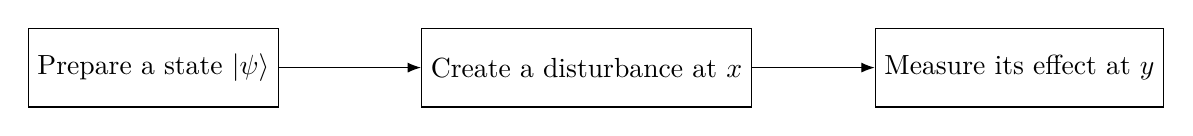
\begin{tikzpicture}[>=Latex,node distance=5.5cm]
            \node[draw, rectangle, minimum width=3cm, minimum height=1cm] (A) {Prepare a state \(\ket{\psi}\)};
            \node[draw, rectangle, right of=A, minimum width=3cm, minimum height=1cm] (B) {Create a disturbance at \(x\)};
            \node[draw, rectangle, right of=B, minimum width=3cm, minimum height=1cm] (C) {Measure its effect at \(y\)};

            % Draw the arrows
            \draw[->] (A) -- (B);
            \draw[->] (B) -- (C);

        \end{tikzpicture}
    \end{figure}
    
    Such questions are answered by computing the correlators of the form — \(\braket{0|\phi(x_1)\cdots\phi(x_n)|0 }\).\\

    However, it turns out that in QFT, although we can ask these questions, a lot of focus is on slightly \textit{simpler} questions.\\
    The simpler question is 
    \begin{figure}[h]
        \centering
        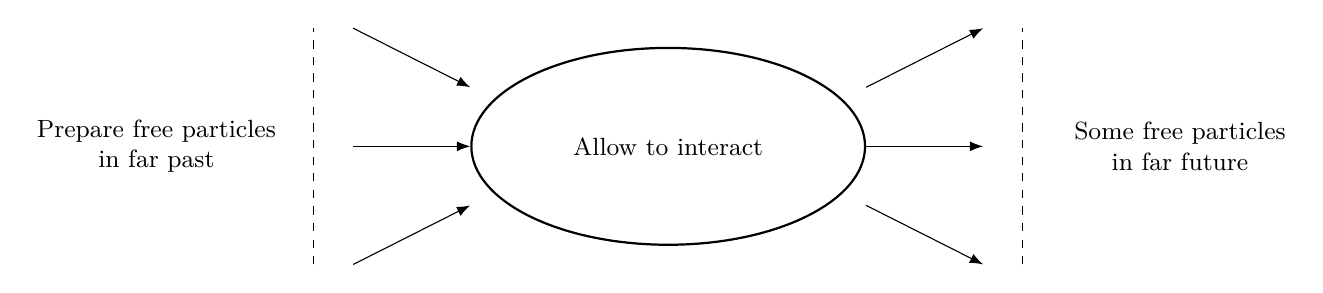
\begin{tikzpicture}[>=Latex, every node/.style={font=\small, align=center}]

            % Left and right text
            \node (in) at (-6.5,0) {Prepare free particles\\in far past};
            \node (out) at ( 6.5,0) {Some free particles \\in far future};

            \draw[dashed] (-4.5, -1.5) -- (-4.5, 1.5);
            \draw[dashed] (4.5, -1.5) -- (4.5, 1.5);

            \node[ellipse, draw, thick,
                minimum width=5cm, minimum height=2.5cm] (proc) 
            at (0,0) {Allow to interact};

            % Converging arrows (left → centre)
            %   start at (-6, +2),(-6,0),(-6,-2)
            %   end at proc.west + (0,+1),(0,0),(0,-1)
            \foreach \sy/\ey in {1.5/0.75, 0/0, -1.5/-0.75} {
                \draw[->] (-4,\sy) -- ($(proc.west)+(0,\ey)$);
            }

            % Diverging arrows (centre → right)
            %   start at proc.east + (0,+1),(0,0),(0,-1)
            %   end at (6,+2),(6,0),(6,-2)
            \foreach \ey/\sy in {0.75/1.5, 0/0, -0.75/-1.5} {
                \draw[->] ($(proc.east)+(0,\ey)$) -- (4,\sy);
            }

        \end{tikzpicture}
    \end{figure}

    That is, we create free particles in far past, let them evolve and interect, and ask what are the free particles and their properties in far future. This kind of question is answered by something called the \(S\) matrix. One might think that this is less general than the other question, but in fact it turns out that it has all the information we want to have about the theory. \\

    Why we talk about \(S\) matrix?
    \begin{enumerate}
        \item Experiments — most physics we learn from experiments is from this kind of experiments. 
        \item Theoretical reasons — two theoretical reasons \begin{itemize}
            \item \(S\) matrix is an unambigously decided observable. That is if we ask the question like what is the correlator 
            \begin{equation*}
                \braket{\psi | \phi(x_1) \cdots \phi(x_n)| \psi}
            \end{equation*}
            this is very ambigous. This is because in interacting theory, there is no unambigous \textit{definition} of field. One can always redefine the fields at the cost of adding interaction terms, without altering the physical content of the theory. When the fields are free and don't interact, there is 'a' free field, and field redefinitions do not obey the equations of motions whereas the original field obeys. But in case of interacting theories, no fields obey the equation of motion, and therefore there is no more unique field.\\
            There is a class of field theories called conformal field theories, where there are other principles that allows one to uniquely identify field variables even in the case of interactions, and there we can talk about the first type of questions. But in general \(S\) matrix is unambigously defined since all we talk about is free theories in far past and future.
            \item In Quantum Gravity, maybe only the \(S\) matrix makes sense. The reason for that is that the first type of questions involve some local questions about what happens in some local regions of spacetime, and when the metric itself is fluctuating and spacetime itself is fluctuating, such questions are not well defined. But when we ask the second type of questions, in far past and future, where such fluctuations are not present, it is perfectly well defined. 
        \end{itemize}
    \end{enumerate}

    Therefore there are good reasons to consider the \(S\) matrix. Now we develop the machinery needed to calculate these \(S\) matrices. 

    \subsection{The Interaction Hamiltonian}
    For an interacting theory, the Hamiltonian looks like 
    \begin{equation*}
        H = H_0 + H_{\text{int}}
    \end{equation*}
    where \(H_0\) is the free part, and \(H_{\text{int}}\) is the interacting part. \\
    To make the intuition more precise, one can also consider adding a \textit{turning on-off function} \(f(t)\) such that 
    \begin{equation*}
        H = H_0 + f(t) H_{\text{int}}
    \end{equation*}
    and \(f(t)\) is such that it starts at \(0\) at \(-\infty\) and it rapidly rises to \(1\), stays \(1\) for a long time, and then dies off rapidly to \(0\) again at \(\infty\). The purpose of this function is to make the Hamiltonian free in far past and far future, while keeping the interactions turned on in between. It is often not necessary to think of this turning on-off function if we talk about the right initial and final states, i.e.\ if we discuss about particles that separate sufficiently as we go in the far future/past, the \textit{turning off} of interactions automatically happens.\\

    If we call fields in the far past \(\phi_{in}\) and fields in far future \(\phi_{out}\), we can take these fields and act them on the vacuum, we can create free particles in far past and far future. We get two Fock spaces, corresponding to \(\phi_{in}\) and \(\phi_{out}\)
    \begin{align*}
        &\mathbb{H}_{in} = \mathrm{span} \{ \ket{0}, \ket{\textbf{k}}, \ket{\textbf{k}_1, \textbf{k}_2}, \cdots \}\\
        &\mathbb{H}_{out} = \mathrm{span} \{ \ket{0}, \ket{\textbf{k}}, \ket{\tilde{\textbf{k}}_1, \tilde{\textbf{k}}_2}, \cdots \}
    \end{align*}
    The vacuum in both the spaces are the same as they both are the vacuum of the same \(H_0\). The one particle states are also the same, as required by the conservation of momentum. However, the higher particle states are not necessarily the same. That is, if we started with a single particle in the far past with momentum \(\textbf{k}\), it is necessary that in the far future the momentum is still \(\textbf{k}\). But this is not the case in case of multi-particle states, where a state with momentum \((\textbf{k}_1, \textbf{k}_2, \cdots)\) can transform into the state \((\tilde{\textbf{k}}_1, \tilde{\textbf{k}}_2, \cdots)\) as long as the energy-momentum is conserved. \\
    We can immediately see that 
    \begin{equation*}
        \indices{_{in}}\braket{0|0}_{out} = 1
    \end{equation*}
    \begin{equation*}
        \indices{_{in}}\braket{\textbf{k} | \tilde{\textbf{k}}}_{out} = (2\pi)^3\delta(\textbf{k} - \tilde{\textbf{k}})
    \end{equation*} 
    and there the non-trivial matrix elements are 
    \begin{equation*}
       \indices{_{in}}\braket{\textbf{k}_1, \textbf{k}_2, \cdots | \tilde{\textbf{k}}_1, \tilde{\textbf{k}}_2, \cdots}_{out}
    \end{equation*}
    where the number of momenta in the in states need not be equal to the number of momenta in the out space. That is, we can have a one particle state going to a two particle state and so on too. \\

    These two \(\mathbb{H}\) spaces should be related by unitary transformation, since we have one description that describes all degrees of freedom in far past and another description for the far future, it is necessary, for the probabilities to be conserved, that they both are related by a unitary transformation. If we tell all the matrix elements we discussed above, we know what the unitary transformation is. And it is this matrix that is called the \(S-\)matrix. The \(S-\)matrix is a particular limit of the correlation functions \(\braket{0|\phi(x_1) \cdots \phi(x_n)|0}\), with some \(t\) taken to \(-\infty\) and some to \(+\infty\), and this limit is given by the LSZ formula. \\

    To compute the \(S-\)matrix, we need the time evolution operator, \(U(-\infty, \infty)\). Obtaining this operator exactly is not possible in most interacting field theories, and therefore we need to resort to a perturbation theory. One tool we use to calculate this is called the interaction picture. 

    \subsection{The Interaction Picture}
    In the Schrodinger picture, the observables do not evolve, but the states evolve. That is 
    \begin{align*}
        \ket{\psi} &\to \e^{-iHt}\ket{\psi}\\
        O &\to O 
    \end{align*}
    In QFT, the observables are the fields, and terefore, we fix a time slice, lets say \(t=0\) and call all the fields \(\phi(0, \textbf{x})\) in this time slice as observables. \\

    In the Heisenberg picture, which is little more natural in field theory, and therefore is the picture in which we had our discussions so far, the states do not evolve, but the operators do. 
    \begin{align*}
        \ket{\psi} &\to \ket{\psi}\\
        O &\to \e^{iHt}O\e^{-iHt}
    \end{align*}
    In this description, as we have already seen, the operators are \(\phi(t, \textbf{x}) \equiv \phi(x)\). This is more natural because we are concerned with observations in different times, and for someone at a later time \(t\), it doesn't make sense to discuss observations in terms of the operators \(\phi(0, \textbf{x})\). \\

    In the interaction picture, we solve exactly for the free part of the Hamiltonian and perturbatively for the interacting part. In this picture, we introduce a new operator 
    \begin{equation*}
        O_I (t) = \e^{iH_0 t}O(0) \e^{-iH_0 t}
    \end{equation*}
    which evolves according to the free Hamiltonian.\\

    To find its relation to the Heisenberg picture operator, we first undo the evolution by free Hamiltonian and then evolve it according to the full Hamiltonian, i.e.
    \begin{equation*}
        O_H(t) =
        \underbrace{e^{i H t} e^{-i H_0 t} }_{U_I^\dagger(t)}
        \;
        \overbrace{e^{i H_0 t}O(0)e^{-i H_0 t}}^{O_I(t)}
        \;
        \underbrace{ e^{i H_0 t} e^{-i H t}}_{U_I(t)}
    \end{equation*}
    \(U_I(t)\) is a unitary operator, but is different from the regular time evolution operator. To see why this is useful, see that the equation of motion it follows is
    \begin{equation*}
        \frac{d}{dt}U_I(t) = \e^{iH_0t}(iH_0)\e^{-iHt} + \e^{iH_0t} (-iH) \e^{-iHt}
    \end{equation*}
    (notice that \(H\) and \(H_0\) do not necessarily commute, also \(H_0\) and \(H_{\text{int}}\) are time independent. It is \((H_0)_I\) and \((H_{\text{int}})_I\) that are time dependent).\\
    This is equal to 
    \begin{align*}
        \frac{d}{dt}U_I(t)&= -i\e^{iH_0t} (H- H_0) \e^{-iHt}\\
        &=-i\e^{iH_0t} (H- H_0) \e^{-iH_0t} \e^{iH_0t}\e^{-iHt}\\
        &=-i(H_{\text{int}})_I(t) U_I(t)
    \end{align*}
    This equation is similar to the one satisfied by the regular time evolution operator, but with \(H_{\text{int}}\) instead of the full Hamiltonian. \\

    To see why this is a very important picture, let us consider adding a term \(\lambda\phi^4(x)\). When we make the split between \(H_0\) and \(H_{\text{int}}\), we need to choose a specific time, since these terms can mix with time when evolved under the full Hamiltonian. Let us therefore consider the splitting at time \(t=0\)
    \begin{equation*}
        H_{\text{int}} = \int d^3\textbf{x} ~\lambda \phi(0, \textbf{x})^4
    \end{equation*}

    For this interaction, 
    \begin{equation*}
        i\frac{d}{dt}U_I(t) = \lambda \e^{iH_0t}  \int d^3\textbf{x} ~\lambda \phi(0, \textbf{x})^4 \e^{-iH_0t} U_I(t)
    \end{equation*}
    But 
    \begin{equation*}
        \e^{iH_0t}  \int d^3\textbf{x} ~\lambda \phi(0, \textbf{x})^4 \e^{-iH_0t} = \int d^3\textbf{x}~\lambda \phi(t, \textbf{x})^4
    \end{equation*}
    where now the fields evolve according to the free Hamiltonian, and we already know the explicit expression for the interaction picture fields at time \(t\). That is, this equation converts everything in terms of interaction picture at time \(t\).\\

    But there is a problem, the equation of motion for the actual time evolution operator depends on \(H\) which is the full Hamiltonian, and is therefore a time independent quantity. But in the above equation \((H_{\text{int}})_I(t)\) is also a time dependent quantity, and therefore we need to treat it carefully.

    \subsection{The Time Evolution Operator}
    In the case of the complete Hamiltonian, the actual time evolution operator also follows
    \begin{equation*}
        \frac{d}{dt}U(t) = -iHU(t)
    \end{equation*}
    In this case, the \(H\) is time independent, and the equation has a solution 
    \begin{equation*}
        U(t) = \e^{-i\int_0^t Hdt'} = \e^{-iHt} \because ~H \text{ is time independent.}
    \end{equation*}
    Let us try to solve the previously discussed equation by (wrongly) assuming that the solution in this case too is an exponential, and seeing where it goes wrong. Let us guess (from now on we simply write \(H_I(t)\) for \((H_\text{int})_I(t)\))
    \begin{equation*}
        U^g(t) = \e^{-i\int_0^{t} H_I(t') dt'}
    \end{equation*} 
    where the superscript \(g\) stands for guess. Expanding this in Taylor series, 
    \begin{equation*}
        U^g(t) = 1 - i\int_0^t H_I(t') dt' - \frac{1}{2} \int_0^t H_I(t') dt' \int_0^t H_I(t'') dt'' + \cdots
    \end{equation*}
    We can now check if this satisfies the above equation by taking the time derivative
    \begin{equation*}
        \frac{d}{dt}U^g(t) = -iH_I(t) - \frac{1}{2} H_I(t) \left(\int_0^t H_I(t')dt'\right) - \frac{1}{2} \left(\int_0^t H_I(t') dt'\right) H_I(t) + \cdots
    \end{equation*}
    Now if \(H_I(t)\) commuted with \(H_I(t')\), we could have moved the \(H_I(t)\) to the left in the third term and add it to the second term to form \(H_I(t) \int_0^t H_I(t')dt'\), and this expression would be the right expression for \(U_I\). But since they do not commute, we cannot do such a manipulation. We face similar problems for all higher order powers, and therefore our guess for the time evolution operator is not the right one.\\

    We can fix this by considering the following expression
    \begin{align*}
        U_I(t) = 1 + (-i)\int_0^t H_I(t') dt' &+ (-i)^2 \int_0^t H_I(t') \int_0^{t'} H_I(t'') dt''dt' \\
        &+ (-i)^3 \int_0^t H_I(t') \int_0^{t'} H_I(t'') \int_0^{t''} H_I(t''')dt'''  dt''dt' \cdots
    \end{align*}
    (The individual integral limits are now changed, they are not all \(t\) anymore. Also there are no \(\frac{1}{n!}\) accompanying each terms). \\
    When differentiating this, we get 
    \begin{align*}
        \frac{d}{dt}U_I(t) &= -i H_I(t) + (-i)^2 H_I(t) \int_0^t H(t'')dt'' + (-i)^3 H_I(t) \int_0^{t} H_I(t'') \int_0^{t''} H_I(t''')dt''' \cdots\\
        &= -iH_I(t) U_I(t)
    \end{align*}
    which is the required equation. \\

    We can rewrite this in a slightly compact way by introducing \textit{time ordering}. The above equation has the property that operators later in time are on the left, i.e. if \(t' > t''\), then in the expansion \(H(t')\) will always be to the left of \(H(t'')\). \\
    
    \textcolor{red}{
        To see this explicitly, consider a discretized version of the double integral of the above form 
        \begin{equation*}
            \sum_0^t H(a) \sum_0^a H(b)
        \end{equation*}
        Upon expanding the series we get 
        \begin{equation*}
            H(0)H(0) + H(1)[H(0) + H(1)] + H(2)[H(0) + H(1) + H(2)] + \cdots + H(t)[H(0) + \cdots + H(t)]
        \end{equation*}
        See that at no point in the entire expansion we had a term of the form \(H(a) H(b)\) with \(a<b\).\\
    }

    It is convenient to introduce the notion of time ordering which is defined as 
    \begin{equation*}
        T(A(t_1, \textbf{x})B(t_2, \textbf{y})) = \begin{cases}
            A(t_1, \textbf{x})B(t_2, \textbf{y}) &: t_1 > t_2\\
            B(t_2, \textbf{y})A(t_1, \textbf{x}) &: t_2 > t_1
        \end{cases}
    \end{equation*}
    Using this, we can write the above expression as 
    \begin{equation*}
        U_I(t) = 1 - i\int_0^t T(H(t')) dt' + (-i)^2 \int_0^t \int_0^{t'} T(H(t')H(t''))dt''dt' + \cdots
    \end{equation*}
    This is the expression we already had above, it was already time ordered, we just made it explicit here, without changing anything. We can see that (considering specifically the double integral), the integral runs \(dt'\) from \(0\) to \(t\), and \(t''\) from \(0\) to \(t'\). That is, we are integrating over the region 
    \begin{figure}[h]
        \centering
        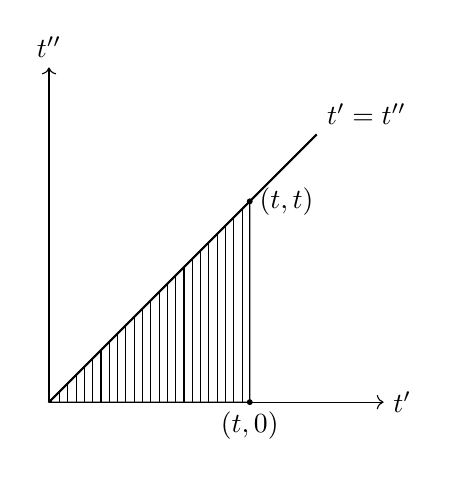
\begin{tikzpicture}[scale=0.85]
            % axes
            \draw[->] (0,0) -- (5,0) node[right] {$t'$};
            \draw[->] (0,0) -- (0,5) node[above] {$t''$};
            % t'=t'' line
            \draw[thick] (0,0) -- (4,4) node[above right] {$t'=t''$};
            % define base length t (adjust as needed)
            \def\t{3}
            % shaded triangle using vertical line pattern
            \draw[pattern=vertical lines,pattern color=black] (0,0) -- (\t,0) -- (\t,\t) -- cycle;
            % optional: mark point at (t,0) and (t,t)
            \filldraw (\t,0) circle (1pt) node[below] {$(t,0)$};
            \filldraw (\t,\t) circle (1pt) node[right] {$(t,t)$};
        \end{tikzpicture}
    \end{figure}

    We can also have the \(t''\) integration to go from \(0\) to \(t\), since we are explicitly enforcing time ordering, we will get the same expression but twice. (Think carefully about this, if there were no time ordering, this manipulation would not be possible, since for the upper triangle, we would be having the products wrongly ordered. The presence of time ordering allows one to extend the integral without altering its value.) Similarly, we can extend all the integrals to \(t\), while being reassured by the time ordering that we are getting consistent results, while dividing by \(n!\) which removes the factor of adding over all the possible arrangements of the \(n\) dummy variables. Therefore, we can write the above also as 
    \begin{equation*}
        U_I(t) = 1 - i\int_0^t T(H(t')) dt' + (-i)^2 \frac{1}{2!}\int_0^t \int_0^t T(H(t')H(t''))dt''dt' + \cdots
    \end{equation*}

    \textcolor{red}{
        Let us again explicitly see this in the case of the discrete sum 
        which now would be rewritten as 
        \begin{equation*}
            \sum_0^t \sum_0^t T(H(a) H(b))
        \end{equation*}
        This would be equal to 
        \begin{align*}
            &\sum_{a>b} H(a)H(b) + \sum_{a<b}H(b)H(a) + \sum_{a=b}H(a)^2
        \end{align*}
        Since the first two sums are equal, we get 
        \begin{equation*}
            2\sum_{a>b} H(a)H(b) + \sum_{a=b}H(a)^2
        \end{equation*}
        In continuum, the diagonal term has zero measure and drops out, and therefore, we will be left with twice the intended integral as expected.\\
    }

    Therefore 
    \begin{equation*}
        U_I(t) = \sum_{n=0}^\infty \frac{(-i)^n}{n!} \left(\int_0^t\right)^n T(H(t_1) H(t_2) \cdots H(t_n)) ~dt_1 dt_2 \cdots dt_n 
    \end{equation*}
    and there is a formal way to write this, called the Dyson's formula
    \begin{equation*}
        U_I(t) = T\left\{ \e^{-i\int_0^t H_I(t')dt'}  \right\}
    \end{equation*}
    What this means is that we expand the exponential in its Taylor series and then apply the time ordering to very term.\\

    Given an operator in terms of the free fields \(\phi_I(t,\textbf{x})\), the above derived \(U_I(t)\) gives us a way to obtain the full Heisenberg picture operators. An inherent advantage is that this formula is already in the form of a power series in \(H_I\), and therefore naturally provides a perturbative series.

    \newpage
    \section{Wick's Theorem}
    In general, what we want to compute is what the matrix elements of the above derived \(U_I(t)\) are, since this gives us the amplitudes for some in states going to some out states. In computing these matrix elements, we have to compute the matrix elements of the kind 
    \begin{equation*}
        \braket{\psi_1 | T[H_I(t_1),\cdots,H_I(t_n)]|\psi_2}
    \end{equation*}
    where \(\ket{\psi_1}\) and \(\ket{\psi_2}\) are the in and out states (we will later formulate these only in terms of vacuum expectation values, but it is more physically relevant to talk about these matrix elements). Once we know all these elements, we can sum them according to the Dyson's formula to get the matrix element of \(U_I\) which gives us the \(S-\)matrix. \\

    The \(H_I(t)\) is some polynomial in \(\phi_I(t, \textbf{x})\), and therefore, the above expectation values reduce to calculating elements of the form 
    \begin{equation*}
        \braket{\psi_1 | T[\phi_I(x_1),\cdots,\phi_I(x_n)]|\psi_2}
    \end{equation*}

    Remember that the interaction picture fields are simply
    \begin{equation*}
        \phi_I(t,\textbf{x}) = \int \a{p}\e^{-ip\cdot x} + \adag{p}\e^{ip\cdot x} \frac{d^3\textbf{p}}{(2\pi)^3 \sqrt{2\w_\textbf{p}}}
    \end{equation*}
    and the above matrix values are simply matrix elements of the time ordered products of the fields of this kind. But see that the time ordered product is going to be a mess, to see why consider a simple case of three field insertions 
    \begin{align*}
        T[\phi(x_1)\phi(x_2)\phi(x_3)] =& ~\theta(x_1^0 - x_2^0)\theta(x_1^0 - x_3^0)\theta(x_2^0 - x_3^0) \phi(x_1)\phi(x_2)\phi(x_3) \\
        &+  \theta(x_2^0 - x_1^0)\theta(x_2^0 - x_3^0)\theta(x_1^0 - x_3^0) \phi(x_2)\phi(x_1)\phi(x_3) \\
        &+ \text{ 4 other terms}
    \end{align*}
    Each of the term above has further \(2^3\) terms since each field insertion has a creation and annihilation operator, and therefore the product of \(n\) such field insertions has \(2^n\) terms. This expression only gets more complicated for polynomials with more field insertions, which is natural in such interaction Hamiltonians, and therefore the entire matrix element is a mess. The tool that is used to simplify this mess is called the Wick's theorem.

    \subsection{Contractions}

    Earlier, we had encountered the normal ordering, which was simply an instruction to place all the annihilation operators on the right. We can extend this definition to the interaction picture field operators by expanding them in terms of creation and annihilation operators and normal order it. That is, 
    \begin{equation*}
        \phi_I(x) = \phi_I^+(x) + \phi_I^-(x)
    \end{equation*}
    where 
    \begin{equation*}
        \phi_I^+(x) = \int \a{p}\e^{-ip\cdot x} \frac{d^3\textbf{p}}{(2\pi)^3 \sqrt{2\w_\textbf{p}}}~~~~\&~~~~\phi_I^-(x) = \int \adag{p}\e^{ip\cdot x} \frac{d^3\textbf{p}}{(2\pi)^3 \sqrt{2\w_\textbf{p}}}
    \end{equation*}
    (which is taken by convention — positive frequency contains the annihilation operators and negative frequency contains the creation operators) then, 
    \begin{align*}
        \normord{\phi_I(x_1) \phi_I(x_2)} &= \normord{\phi_I^+(x_1)\phi_I^+(x_2)} + \normord{\phi_I^+(x_1)\phi_I^-(x_2)} + \normord{\phi_I^-(x_1)\phi_I^+(x_2)} + \normord{\phi_I^-(x_1)\phi_I^-(x_2)}\\
        &= \phi_I^+(x_1)\phi_I^+(x_2) + \phi_I^-(x_2)\phi_I^+(x_1) + \phi_I^-(x_1)\phi_I^+(x_2) + \phi_I^-(x_1)\phi_I^-(x_2)
    \end{align*}
    (where only the second term is different from the regular product)
    Notice that normal ordered product is NOT defined for operators in Heisenberg picture since in Heisrnberg picture in the presence of interactions, there is no splitting of the field into creation and annihilation operators. This ordering is only valid for interactin picture fields\\

    We define a contraction as 
    \begin{equation*}
        \wick{\c \phi_I(x_1) \c \phi_I(x_2)} = T[\phi_I(x_1) \phi_I(x_2)] - \normord{\phi_I(x_1) \phi_I(x_2)}
    \end{equation*}
    The normal ordered product and time ordered product are operators, but contraction is just a number. We know that 
    \begin{equation*}
        T[\phi_I(x_1) \phi_I(x_2)] = \theta(x_1^0 - x_2^0) \phi_I(x_1) \phi_I(x_2) + \theta(x_2^0 - x_1^0) \phi_I(x_2) \phi_I(x_1)
    \end{equation*}
    and the normal ordered product is 
    \begin{equation*}
        \normord{\phi_I(x_1) \phi_I(x_2)} = \phi_I^+(x_1)\phi_I^+(x_2) + \phi_I^-(x_2)\phi_I^+(x_1) + \phi_I^-(x_1)\phi_I^+(x_2) + \phi_I^-(x_1)\phi_I^-(x_2)
    \end{equation*}
    we can simply insert a \(\theta\) function in the normal ordered product without altering it as 
    \begin{align*}
        \normord{\phi_I(x_1) \phi_I(x_2)} =& \theta(x_1^0 - x_2^0)\left[ \phi_I^+(x_1)\phi_I^+(x_2) + \phi_I^-(x_2)\phi_I^+(x_1) + \phi_I^-(x_1)\phi_I^+(x_2) + \phi_I^-(x_1)\phi_I^-(x_2) \right] \\
         &+ \theta(x_2^0 - x_1^0)\left[ \phi_I^+(x_1)\phi_I^+(x_2) + \phi_I^-(x_2)\phi_I^+(x_1) + \phi_I^-(x_1)\phi_I^+(x_2) + \phi_I^-(x_1)\phi_I^-(x_2) \right]
    \end{align*}
    Then the difference in the two products would be (noticing that the only different term is the second term in the normal ordering)
    \begin{align*}
        \wick{\c \phi_I(x_1) \c \phi_I(x_2)} &= \theta(x_1^0 - x_2^0)\left( \phi_I^+(x_1)\phi_I^-(x_2) - \phi_I^-(x_2)\phi_I^+(x_1) \right) + \theta(x_2^0 - x_1^0) \left(  \phi_I^+(x_2)\phi_I^-(x_1) - \phi_I^-(x_1)\phi_I^+(x_2)  \right)\\
        &=\theta(x_1^0 - x_2^0) [\phi_I^+(x_1), \phi_I^-(x_2)] + \theta(x_2^0 - x_1^0) [\phi_I^+(x_2), \phi_I^-(x_1)] 
    \end{align*}
    These commutators are only numbers, and not operators.

    \subsection{The theorem}

    Wick's theorem simply tell that 
    
    \begin{equation}
            \begin{split}
                T[\phi_I(x_1) \phi_I(x_2)& \cdots \phi_I(x_n)] = \normord{\phi_I(x_1) \phi_I(x_2) \cdots \phi_I(x_n)} + \normord{\wick{\c \phi_I(x_1) \c \phi_I(x_2)} \cdots \phi_I(x_n)} \\
                &+ \normord{\wick{\c \phi_I(x_1) \phi_I(x_2)\c \phi_I(x_3)} \cdots \phi_I(x_n)} + \text{ other terms with 1 contraction}\\
                &+ \normord{\wick{\c1 \phi_I(x_1) \c1 \phi_I(x_2) \c1 \phi_I(x_3) \c1 \phi_I(x_4)} \cdots \phi_I(x_n)} + \text{ other terms with 2 contractions}\\
                &+ \cdots \text{ terms with 3 and more contractions}\\
                &+ \begin{cases}
                    \normord{\wick{\c1 \phi_I(x_1) \c1 \phi_I(x_2) \cdots \c1 \phi_I(x_{n-2}) \c1 \phi_I(x_{n-1})} \phi_I(x_n)} + \text{terms with only one uncontracted field } : n \text{ odd}\\
                    \normord{\wick{\c1 \phi_I(x_1) \c1 \phi_I(x_2) \cdots \c1 \phi_I(x_{n-1}) \c1 \phi_I(x_{n})}} + \text{terms with no uncontracted field } : n \text{ even}
                \end{cases}
            \end{split}
            \label{eq:wick}
    \end{equation}
    As an example, 
    \begin{align*}
        T[\phi_I(x_1) \phi_I(x_2) \phi_I(x_3)\phi_I(x_4)] =& \normord{\phi_I(x_1) \phi_I(x_2) \phi_I(x_3)\phi_I(x_4)} + \normord{\wick{\c\phi_I(x_1) \c\phi_I(x_2) \phi_I(x_3)\phi_I(x_4)}}\\
        &+\normord{\wick{\c\phi_I(x_1) \phi_I(x_2)\c \phi_I(x_3)\phi_I(x_4)}} + \normord{\wick{\c\phi_I(x_1)\phi_I(x_2) \phi_I(x_3)\c\phi_I(x_4)}}\\
        &+\normord{\wick{\phi_I(x_1) \c\phi_I(x_2) \c\phi_I(x_3)\phi_I(x_4)}}+\normord{\wick{\phi_I(x_1) \c\phi_I(x_2) \phi_I(x_3)\c\phi_I(x_4)}}\\
        &+\normord{\wick{\phi_I(x_1) \phi_I(x_2) \c\phi_I(x_3) \c\phi_I(x_4)}} + \normord{\wick{\c \phi_I(x_1) \c \phi_I(x_2) \c\phi_I(x_3) \c\phi_I(x_4)}} \\
        &+\normord{\wick{\c\phi_I(x_1) \c2\phi_I(x_2) \c\phi_I(x_3) \c2\phi_I(x_4)}}
    \end{align*}

    \underline{Proof}\\
    We prove the theorem by induction.\\
    For \(n=2\), the theorem is definitely true, by the definition of contraction.\\
    Suppose the theorem is true for some \(n\). That is 
    \begin{equation*}
        T[\phi_I(x_1)\cdots\phi_I(x_n)] = W(x_1, \cdots, x_n)
    \end{equation*}
    where we used \(W\) as the shorthand for the RHS in equation (\ref{eq:wick})\\
    For \(n+1\), let us assume without loss of generality that \(x_1^0\) is the latest time. We can do this because inside the \(T\) all operators commute, since at the end \(T\) rearranges them according to their time ordering, and therefore, we can bring the field with the latest time to the first and call it \(\phi_I(x_1)\). Then 
    \begin{equation*}
        T(\phi_I(x_1)\phi_I(x_2) \cdots \phi_I(x_{n+1})) = \phi_I(x_1)T(\phi_I(x_2) \cdots \phi_I(x_{n+1})) 
    \end{equation*}
    From our assumption that the theorem is true for \(n\), \(T(\phi_I(x_2) \cdots \phi_I(x_{n+1}) )= W(x_2, \cdots x_{n+1})\). Now 
    \begin{equation*}
        \phi_I(x_1) = \phi_I^+(x_1) + \phi_I^-(x_1)
    \end{equation*} 
    which means 
    \begin{equation*}
        T(\phi_I(x_1)\phi_I(x_2) \cdots \phi_I(x_{n+1})) = (\phi_I^-(x_1) + \phi_I^+(x_1))W(x_2, \cdots x_{n+1}) 
    \end{equation*}
    The first term in the RHS is already has \(\phi^-\) on the left, but the second term is not normal ordered. Therefore, we can commute the \(\phi^+\) to normal order the second term too as
    \begin{equation*}
        T(\phi_I(x_1)\phi_I(x_2) \cdots \phi_I(x_{n+1})) = \phi_I^-(x_1)W(x_2, \cdots x_{n+1}) + W(x_2, \cdots x_{n+1})\phi_I^+(x_1) + [\phi_I^+(x_1), ~W(x_2, \cdots x_{n+1})]
    \end{equation*} 
    The first two terms when added together simply gives 
    \begin{equation*}
        \normord{\phi_I(x_1) W(x_2, \cdots x_{n+1})}
    \end{equation*}
    which is the set of \(\normord{\phi_I(x_1) \phi_I(x_2) \cdots \phi_I(x_{n+1})}\) and all terms with \(\phi_I(x_1)\) uncontracted. \\

    The next part, which is the commutator, will have terms of the form 
    \begin{equation*}
        [\phi_I^+(x_1), \phi_I(x_m)] = [\phi_I^+(x_1), \phi^-_I(x_m)]~ \because \phi^+\text{ at different spacetime points commute}
    \end{equation*}
    But since \(x_1^0 > x_m^0\forall m\), we can also rewrite this as
    \begin{equation*}
        \theta(x_1^0 - x_m^0)[\phi_I^+(x_1), \phi^-_I(x_m)] + \theta(x_m^0 - x_1^0)[\phi_I^+(x_m), \phi^-_I(x_1)] = \wick{\c\phi_I(x_1) \c\phi_I(x_m)}
    \end{equation*} 
    Therefore, the second part will have contractions of \(\phi_I(x_1)\) with all \(\phi_I(x_m)\). \\

    The sum of the first and second part will have everything that is required in \(W(x_1, \cdots, x_{n+1})\), i.e.\ there is a normal ordered product, plus all possible contractions of all fields. Therefore, for \(n+1\)
    \begin{equation*}
        T(\phi_I(x_1)\phi_I(x_2) \cdots \phi_I(x_{n+1})) = W(x_1, \cdots, x_{n+1})
    \end{equation*}
    Therefore, Wick's theorem is proved by mathematical induction.\\

    What makes Wick's theorem useful, and therefore significant, is that it makes evaluation of these time ordered products simple. Suppose we were calculating the vacuum expectation values of a given \(T(\phi_I(x_1)\cdots\phi_I(x_n))\). The only contribution would be from the terms where all the fields are contracted, since other terms are normal ordered and normal ordered products annihilate vacuum and therefore have zero vacuum expectation values. 

    \subsection{The Feynman Propagator}
    See that 
    \begin{equation*}
        \braket{0|T(\phi_I(x) \phi_I(y))|0} = \braket{0|\wick{\c \phi_I(x) \c \phi_I(y)} |0} = \wick{\c \phi_I(x) \c \phi_I(y)} 
    \end{equation*}
    Since the normal ordered product annihilates the vacuum, contraction is a number, and \(\braket{0|0} = 1\).\\

    For \(x^0 > y^0\), this evaluates to 
    \begin{equation*}
        \int \bra{0} \a{q} \e^{-iq\cdot x} \adag{p}\e^{ip\cdot y} \ket{0} \frac{d^3\textbf{p}d^3\textbf{q}}{(2\pi)^6 2\sqrt{\w_\textbf{p}\w_\textbf{q}}}
    \end{equation*}
    since all other terms give zero. We can now commute the \(a\) and \(\adag{}\) to get a delta function, which removes one integral in \(\textbf{q}\), and obtain 
    \begin{equation*}
        \int \e^{-ip\cdot(x-y)}\frac{1}{2\w_\textbf{p}} \frac{d^3\textbf{p}}{(2\pi)^3}
    \end{equation*}
    When \(y^0 > x^0\), we similarly get 
    \begin{equation*}
        \int \e^{ip\cdot(x-y)}\frac{1}{2\w_\textbf{p}} \frac{d^3\textbf{p}}{(2\pi)^3}
    \end{equation*}
    and therefore the contraction looks like 
    \begin{equation}
        \wick{\c \phi_I(x) \c \phi_I(y)} = \theta(x^0 - y^0) \int \e^{-ip\cdot(x-y)}\frac{1}{2\w_\textbf{p}} \frac{d^3\textbf{p}}{(2\pi)^3} ~~+~~\theta(y^0-x^0) \int \e^{ip\cdot(x-y)}\frac{1}{2\w_\textbf{p}} \frac{d^3\textbf{p}}{(2\pi)^3}
        \label{eq:contraction-full}
    \end{equation}

    We can write it in a slighly simpler way as 
    \begin{equation}
        \wick{\c \phi_I(x) \c \phi_I(y)}  = \int\frac{i}{p^2 - m^2 + i\epsilon} \e^{-ip\cdot(x-y)}\frac{d^4p}{(2\pi)^4} = \int \e^{-ip_0 (x^0 - y^0)} \e^{i\textbf{p}\cdot (\textbf{x}- \textbf{y})} \frac{i}{p_0^2 - \textbf{p}^2 - m^2 + i\epsilon} \frac{dp_0 d^3\textbf{p}}{(2\pi)^4}
        \label{eq:feynman}
    \end{equation}
    The \(i\epsilon\) is just a prescription to indicate in which direction the contour should be closed. See that when we do the integral over \(p_0\) without the \(i\epsilon\) shifting, it has two poles, 
    \begin{equation*}
        p_0^2 - \textbf{p}^2 - m^2 = 0 \implies p_0 = \pm \w_\textbf{p}
    \end{equation*}
    on the real axis and therefore the integral is ill defined. The \(i\epsilon\) shifts the poles in such a way that taking a contour along the real axis and closing the contour along one of the two half planes will give the correct result.\\


    With the introduction of \(i\epsilon\), the poles now move to 
    \begin{equation*}
        p_0 = \pm \sqrt{\w_\textbf{p}^2 - i\epsilon} \approx \pm \left( \w_\textbf{p} - \frac{i\epsilon}{2\w_\textbf{p}} \right) \approx \pm (\w_\textbf{p} - i\epsilon)
    \end{equation*}
    (notice that the \(i\epsilon\) is simply an integral prescription and its value has no meaning). Therefore, for the \(p_0\) integral the location of poles is shown in figure (\ref{fig:prescription})
    \begin{figure}[h]
        \centering
        \begin{tikzpicture}[>=latex, scale=1]
            \draw[->] (-3,0) -- (3,0);
            \draw[->] (0, -1.5) -- (0,1.5);
            \fill (1.5,0) circle (2pt);
            \node at (-1.5, -0.25) {\(-\w_\textbf{p}\)};
            \node at (1.5, 0.25) {\(\w_\textbf{p}\)};
            \fill (-1.5,0) circle (2pt);

            \node at (1.5, -1.2) {\(\w_\textbf{p} - i\epsilon\)};
            \node at (1.5, -0.75) {\(\mathsf{X}\)};
            \node at (-1.5, 1.2) {\(-\w_\textbf{p} + i\epsilon\)};
            \node at (-1.5, 0.75) {\(\mathsf{X}\)};

            \begin{scope}[xshift=7cm]
                \draw[->, opacity=0.35] (-3,0) -- (3,0);
                \draw[->, opacity=0.35] (0, -1.5) -- (0,1.5);
                \fill (1.5,0) circle (2pt);
                \node at (-1.5, 0.25) {\(-\w_\textbf{p}\)};
                \node at (1.5, -0.25) {\(\w_\textbf{p}\)};
                \fill (-1.5,0) circle (2pt);
                \draw[->] (1,0) arc (180:0:0.5);
                \draw[<-] (-1,0) arc (360:180:0.5);
                \draw[->] (-1,0) -- (1,0);
                \draw (2,0) -- (3,0);
                \draw (-2,0) -- (-3,0);
            \end{scope}
        \end{tikzpicture}
        \caption{The position of poles in case of \(i\epsilon\) prescription (left), and the equivalent contour we need to consider when working without the shifting (right)}\label{fig:prescription}
    \end{figure}

    To check that this expression with this pole prescription gives the correct result, consider the two cases\\

    1.\ \(x_0 > y_0\)\\
    The integrand is 
    \begin{equation*}
        \e^{-ip_0(x^0 - y^0)} = \e^{-i\mathrm{Re}(p_0) (x^0 - y^0)}\e^{\mathrm{Im}(p_0)(x^0 - y^0)}
    \end{equation*}
    In the upper half of the complex plane, this blows at \(|p_0| \to \infty\) and therefore we close the contour in lower half of the complex plane, picking up the pole at \(\w_\textbf{p} - i\epsilon\). The contour is closed in clockwise sense and the value of the integral is  
    \begin{equation*}
        -2\pi i\frac{1}{2\w_\textbf{p}}\e^{-i\w_\textbf{p}(x^0 - y^0)}
    \end{equation*}
    When plugging the value of this integral into the equation (\ref{eq:feynman}) where one factor of \(2\pi\) cancels with the \((2\pi)^4\) in denominator, and \(-i\) multiplies with \(i\) to give \(1\), we get 
    \begin{equation*}
        \int \e^{-ip\cdot(x-y)}\frac{1}{2\w_\textbf{p}} \frac{d^3\textbf{p}}{(2\pi)^3}
    \end{equation*}
    
    2.\ \(x_0 < y_0\)\\
    In this case the integrand is zero at infinity in the upper half plane and therefore we complete the contour in the upper half plane, picking up the pole at \(p_0 = -\w_\textbf{p}\). The contour is closed counterclockwise, and therefore the integral is 
    \begin{equation*}
        (2\pi i)(-1)\frac{1}{2\w_\textbf{p}}\e^{i\w_\textbf{p}(x^0 - y^0)}
    \end{equation*}
    Plugging this back, we get 
    \begin{equation*}
        \int \e^{i\w_\textbf{p}\cdot(x_0-y_0) + i\textbf{p}\cdot(\textbf{x} - \textbf{y})}\frac{1}{2\w_\textbf{p}} \frac{d^3\textbf{p}}{(2\pi)^3}
    \end{equation*}
    We can convert the integral from \(\textbf{p}\) to \(-\textbf{p}\) to get 

    \begin{equation*}
        \int \e^{ip\cdot(x-y)}\frac{1}{2\w_\textbf{p}} \frac{d^3\textbf{p}}{(2\pi)^3}
    \end{equation*}

    Therefore we recover
    \begin{equation*}
        \wick{\c \phi_I(x) \c \phi_I(y)} = G_F(x-y) =  \begin{cases}
            \displaystyle\int \e^{-ip\cdot(x-y)}\frac{1}{2\w_\textbf{p}} \frac{d^3\textbf{p}}{(2\pi)^3} &: x_0 > y_0\\
            \displaystyle\int \e^{ip\cdot(x-y)}\frac{1}{2\w_\textbf{p}} \frac{d^3\textbf{p}}{(2\pi)^3} &: x_0 < y_0
        \end{cases}
    \end{equation*}
    as required. This is called the Feynman Green's function (Feynman Propagator). (Notice that it was very important to consider \(+i\epsilon\) in the denominator. Any other addition would not give this result.)\\

    There is another way to understand this \(i\epsilon\) prescription as 
    \begin{equation*}
        \frac{1}{x - a - i\epsilon} = P\left( \frac{1}{x-a} \right) + i\pi \delta(x-a)
    \end{equation*}
    where \(P()\) stands for the principle value. The above equation is, in essence, a distribution valued equation, and it makes sense only under an integral 
    \begin{equation*}
        \int \frac{f(x)}{x-a-i\epsilon} dx = P\int \frac{f(x)}{x-a} dx + i\pi f(a) =\lim_{\delta \to 0} \left(\int_{-\infty}^{a-\delta} \frac{f(x)}{x-a} dx+ \int_{a+\delta}^{\infty} \frac{f(x)}{x-a} dx \right) + i\pi f(a)
    \end{equation*}

    To prove this, let us consider the equation
    \begin{equation*}
        \frac{1}{x-a-i\epsilon} - \frac{1}{x-a+i\epsilon} = 2i\pi\delta(x-a)
    \end{equation*}
    which we obtained from adding the above equation to its complex conjugate.\\
    This is equivalent to stating that 
    \begin{equation*}
        \int dx \frac{f(x)}{x-a-i\epsilon} - \int dx \frac{f(x)}{x-a+i\epsilon} = 2i\pi f(a)
    \end{equation*}

    The first term in the above equation simply implies the choice of the contour 
    \begin{figure}[h]
        \centering
        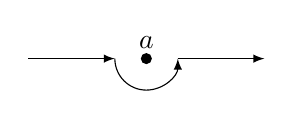
\begin{tikzpicture}[>=latex, scale=1]
            \draw[->] (-1.5, 0) -- (-0.4,0);
            \draw[<-] (1.5, 0) -- (0.4,0);
            \draw[->] (-0.4,0) arc (180:360:0.4);
            \fill (0,0) circle (2pt);
            \node at (0,0.2) {\(a\)};
        \end{tikzpicture}
    \end{figure}

    and the second term implies the choice of the contour 
    \begin{figure}[h]
        \centering
        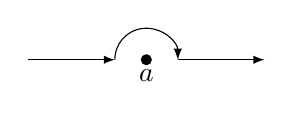
\begin{tikzpicture}[>=latex, scale=1]
            \draw[->] (-1.5, 0) -- (-0.4,0);
            \draw[<-] (1.5, 0) -- (0.4,0);
            \draw[->] (-0.4,0) arc (180:0:0.4);
            \fill (0,0) circle (2pt);
            \node at (0,-0.2) {\(a\)};
        \end{tikzpicture}
    \end{figure}

    Subtracting the above two is equivalent to reversing the direction of the second contour and adding, in which case the only piece that remains is 
    \begin{figure}[h]
        \centering
        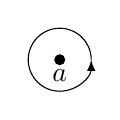
\begin{tikzpicture}[>=latex, scale=1]
            \draw[->] (0.4,0) arc (0:360:0.4);
            \fill (0,0) circle (2pt);
            \node at (0,-0.2) {\(a\)};
        \end{tikzpicture}
    \end{figure}

    which is equal to \(2\pi i\) times the residue of the function at \(x=a\), which is exactly equal to \(2\pi i f(a)\).\\

    Notice that the Feynman progagator also satisfies 
    \begin{equation*}
        (\square + m^2) \braket{0|T(\phi_I(x) \phi_I(y))|0} = -i\delta^4(x-y)
    \end{equation*}

    \textcolor{red}{
        \begin{align*}
                \braket{0|T(\phi_I(x) \phi_I(y))|0} &= \int\frac{i}{p^2 - m^2 + i\epsilon} \e^{-ip\cdot(x-y)}\frac{d^4p}{(2\pi)^4} \\
                \implies (\square + m^2) \braket{0|T(\phi_I(x) \phi_I(y))|0} &= (\square + m^2) \int\frac{i}{p^2 - m^2 + i\epsilon} \e^{-ip\cdot(x-y)}\frac{d^4p}{(2\pi)^4} \\
                &= \int \frac{i}{p^2 - m^2 + i\epsilon} ((-ip)^2 + m^2) \e^{-ip\cdot(x-y)}\frac{d^4p}{(2\pi)^4}\\
                &= -i \int \e^{-ip\cdot(x-y)}\frac{d^4p}{(2\pi)^4}\\
                &= -i\delta^4(x-y)
        \end{align*}
    }
    
    The Feynman propagator has the property that it propagates positive frequencies forward in time, and negative frequencies backwards in time. To see what this means, see that from equation (\ref{eq:contraction-full}), we see that the Feynman propagator is of the form 
    \begin{equation*}
        \int \theta(x^0 - y^0)  \e^{-ik\cdot (x-y)} \theta(k^0) f(k) \frac{d^4k}{(2\pi)^4}  + \int \theta(y^0 - x^0)  \e^{-ik\cdot (x-y)} \theta(-k^0) f(k) \frac{d^4k}{(2\pi)^4}
    \end{equation*}
    (where \(f(k)\) is the \(delta(k^2 - m^2)\), and in the above equation we have simply taken equation (\ref{eq:contraction-full}) and converted it into a manifestly Lorentz invarent \(4-\)integral).\\
    In the second integral, rather than writing the conversion as \(\e^{ik\cdot(x-y)} \theta(k^0) f(k)\), we wrote it as \(\e^{-ik\cdot(x-y)}\theta(-k^0)f(k)\) and used the invariance of the \(3-\)integral under \(\textbf{k}\to -\textbf{k}\). \\
    The propagator in this form has the combinations \(\theta(x^0 - y^0)\theta(k^0)\) and \(\theta(y^0 - x^0)\theta(-k^0)\) which imply that the Feynman propagator propagates positive frequencies forward in time and negative frequencies backward in time.\\

    Feynman propagator is one kind of propagator. We could have considered an anti-time ordered propagator, which would come with a \(-i\epsilon\), and would have the opposite baheviour, propagating positive frequencies backward in time and negative frequencies forward in time. Then there are other propagators which send both the frequencies either backwards or forwards.

    \subsection{The retarded propagator}
    The retarded propagator is simply 
    \begin{equation*}
        \theta(x^0 - y^0)\bra{0}[\phi_I(x), \phi_I(y) ]\ket{0} = G_R(x-y)
    \end{equation*}
    Notice that this propagator also satisfies 
    \begin{equation*}
        (\square + m^2)G_R(x-y) = -i\delta^4(x-y)
    \end{equation*}
    This implies that \(G_F\) and \(G_R\) should differ by only a solution of the equation of motion. To check that this is true, notice that 
    \begin{equation*}
        \frac{\del}{\del x^0} \left(\theta(x^0 - y^0)\bra{0}[\phi_I(x), \phi_I(y) ]\ket{0}\right) = \delta(x^0 - y^0)\bra{0}[\phi_I(x), \phi_I(y) ]\ket{0} + \theta(x^0 - y^0)\frac{\del}{\del x^0} \bra{0}[\phi_I(x), \phi_I(y) ]\ket{0}
    \end{equation*}
    The first term is zero, since at equal times, the fields commute and the delta function enforces equal time. 
    Therefore we get 
    \begin{equation*}
        \frac{\del}{\del x^0} \left(\theta(x^0 - y^0)\bra{0}[\phi_I(x), \phi_I(y) ]\ket{0}\right) = \theta(x^0 - y^0) \bra{0}[\dot{\phi}_I(x), \phi_I(y) ]\ket{0}
    \end{equation*}
    The second derivative w.r.to \(x^0\) would therefore be 
    \begin{align*}
        \frac{\del^2}{\del (x^0)^2} \left(\theta(x^0 - y^0)\bra{0}[\phi_I(x), \phi_I(y) ]\ket{0}\right) &= \delta(x^0 - y^0) \bra{0}[\Pi_I(x), \phi_I(y) ]\ket{0} + \theta(x^0 - y^0) \bra{0}[\ddot{\phi}_I(x), \phi_I(y) ]\ket{0} \\
        &= -i\delta(x^0 - y^0)\delta^3(\textbf{x} - \textbf{y}) + \theta(x^0 - y^0) \bra{0}[\ddot{\phi}_I(x), \phi_I(y) ]\ket{0} 
    \end{align*}
    where in the first term the delta function imposed equal times, and therefore the commutator becomes simply an equal time commutation relation. \\

    There are other terms which are \((-\nabla_x^2 + m^2) G_R\). The \(\nabla_x\) doesn't care about the \(\theta\) function and therefore we would simply get 
    \begin{equation*}
        (-\nabla_x^2 + m^2) \left(\theta(x^0 - y^0)\bra{0}[\phi_I(x), \phi_I(y) ]\ket{0}\right) = \theta(x^0 - y^0)\bra{0}[(-\nabla_x^2 + m^2)\phi_I(x), \phi_I(y) ]\ket{0}
    \end{equation*}
    Adding this and the above equation, we see that we get 
    \begin{equation*}
        (\square + m^2)\left(\theta(x^0 - y^0)\bra{0}[\phi_I(x), \phi_I(y) ]\ket{0}\right) = -i\delta(x^0 - y^0)\delta^3(\textbf{x} - \textbf{y}) + \theta(x^0 - y^0) \bra{0}[(\square + m^2)\phi_I(x), \phi_I(y) ]\ket{0}
    \end{equation*}
    But since \((\square + m^2)\phi_I(x) = 0\), we get 
    \begin{equation*}
        (\square + m^2)\left(\theta(x^0 - y^0)\bra{0}[\phi_I(x), \phi_I(y) ]\ket{0}\right) = -i\delta(x^0 - y^0)\delta^3(\textbf{x} - \textbf{y}) = -i\delta^4(x-y)
    \end{equation*}

    Let us try evaluating this expression in momentum space, the propagator becomes 
    \begin{align*}
        \theta(x^0 - y^0)[\phi_I(x), \phi_I(y)] &= \int \left(  [\a{q}, \adag{p}] \e^{-iq\cdot x + ip\cdot y} + [\adag{q}, \a{p}]\e^{iq\cdot x - ip\cdot y}  \right)\frac{d^3\textbf{p}d^3\textbf{q}}{(2\pi)^62\sqrt{\w_\textbf{p}\w_\textbf{q}}}\\
        &= \int \e^{-iq\cdot(x-y)} - \e^{iq\cdot (x-y)} \frac{d^3\textbf{q}}{(2\pi)^32\w_\textbf{q}}\theta(x^0 - y^0)
    \end{align*}
    Claim - the whole retarded propagator can be written as 
    \begin{equation*}
        G_R(x-y) = \int \frac{i}{(k_0 + i\epsilon)^2 - \textbf{k}^2 - m^2} \e^{-ik\cdot(x-y)} \frac{d^4k}{(2\pi)^4}
    \end{equation*}
    In this case, the poles are at \(k^0 = \pm \w_\textbf{k} - i\epsilon\).

    \begin{figure}[h]
        \centering
        \begin{tikzpicture}[>=latex, scale=1]
            \draw[->] (-3,0) -- (3,0);
            \draw[->] (0, -1.5) -- (0,1.5);
            \fill (1.5,0) circle (2pt);
            \node at (-1.5, 0.25) {\(-\w_\textbf{k}\)};
            \node at (1.5, 0.25) {\(\w_\textbf{k}\)};
            \fill (-1.5,0) circle (2pt);

            \node at (1.5, -1.2) {\(\w_\textbf{p} - i\epsilon\)};
            \node at (1.5, -0.75) {\(\mathsf{X}\)};
            \node at (-1.5, -1.2) {\(-\w_\textbf{p} + i\epsilon\)};
            \node at (-1.5, -0.75) {\(\mathsf{X}\)};

            \begin{scope}[xshift=7cm]
                \draw[->, opacity=0.35] (-3,0) -- (3,0);
                \draw[->, opacity=0.35] (0, -1.5) -- (0,1.5);
                \fill (1.5,0) circle (2pt);
                \node at (-1.5, -0.25) {\(-\w_\textbf{p}\)};
                \node at (1.5, -0.25) {\(\w_\textbf{p}\)};
                \fill (-1.5,0) circle (2pt);
                \draw[->] (1,0) arc (180:0:0.5);
                \draw[->] (-2,0) arc (180:0:0.5);
                \draw[->] (-1,0) -- (1,0);
                \draw (2,0) -- (3,0);
                \draw (-2,0) -- (-3,0);
            \end{scope}
        \end{tikzpicture}
        \caption{The position of the shifted poles (left), and the equivalent contour (right).}
    \end{figure}
    
    For \(x^0 < y^0\), we need to close the contour in the upper half plane, where it does not enclose any poles. Therefore the integral is zero. \\

    For \(x^0 > y^0\), we close the contour in the lower half plane, picking up residues of both the poles. The residues are the same as we had calculated for the case of Feynman propagator, and therefore the above integral for \(x^0 > y^0\) becomes
    \begin{equation*}
        (-2\pi i ) \frac{i}{2\pi} \left(\int \e^{-ik\cdot(x-y)}\frac{1}{2\w_\textbf{k}} \frac{d^3\textbf{k}}{(2\pi)^3} + \int \e^{ik\cdot(x-y)}\frac{1}{-2\w_\textbf{k}} \frac{d^3\textbf{k}}{(2\pi)^3} \right)
    \end{equation*}
    therefore giving 
    \begin{equation*}
        G_R(x-y) = \int \frac{i}{(k_0 + i\epsilon)^2 - \textbf{k}^2 - m^2} \e^{-ik\cdot(x-y)} \frac{d^4k}{(2\pi)^4} = \theta(x^0 - y^0) \int \e^{-ik\cdot(x-y)}\frac{1}{2\w_\textbf{k}} {(2\pi)^3} - \e^{ik\cdot(x-y)}\frac{1}{2\w_\textbf{k}} \frac{d^3\textbf{k}}{(2\pi)^3}
    \end{equation*}
    as required.\\

    There is also an advanced propagator, with \(\theta(y^0-x^0)\) and for this case the pole prescription would be \((k_0 + i\epsilon)^2 - \textbf{k}^2 - m^2\).\\

    The retarded propagator is the propagator we study in classical electrodynamics. To understand why this is the case, we need to understand the physical interpretation of this propagator. In QM, we are allowed to turn on sources for fields. These sources are unitary operators. Say we turn on source, which is equivalent to saying that we do 
    \begin{equation*}
        \ket{\psi} \to \e^{i\int d^4y J(y) \phi(y)} \ket{\psi}
    \end{equation*}
    that is, we add the term \(J(y) \phi(y)\) to the Hamiltonian, with \(J(y)\) controlling the strenght and duration of the current. (This is basically saying that we create excitations in a spacetime, whose strength and the region of excitation are defined by \(J\)). We can now measure the effect at \(x\), which is basically seeing how much the following expectation value deviates from  \(\braket{\psi | \phi(x) | \psi}\)
    \begin{equation*}
        \bra{\psi} \e^{-i\int d^4y J(y) \phi(y) } \phi(x) \e^{i\int d^4y J(y) \phi(y) dy} \ket{\psi}
    \end{equation*}
    The zeroth order term is \(\braket{\psi | \phi(x) | \psi}\) itself, and the first order term is 
    \begin{equation*}
        \int d^4y J(y) \theta(x_0 - y_0)\bra{\psi}[\phi(x), \phi(y)]\ket{\psi}
    \end{equation*}
    Physically, what we are doing is adding a source at \(y\) and measuring its effect at \(x\). Causality requires that there cannot be any effect if \(y_0 > x_0\), which brings a \(\theta\) function. Therefore, the effect is, upto first order 
    \begin{equation*}
        \int d^4y J(y) G_R(x-y) 
    \end{equation*}
    which is the retarded Green's function. (Notice that the above discussion was not precise. To make it precise we need to consider the time ordered exponential as the unitary operator, in which case the \(\theta\) function naturally emerges. The above discussion is purely for extracting physical insights). Therefore, \(G_R(x-y)\) is the linear response at \(x\) to a disturbance at \(y\). This is exactly what we do in Classical Mechanics, where we do a disturbance and measure its affect at some different time and different region.

    \subsection{Wightman Functions}
    They are simply 
    \begin{equation*}
        \bra{0}\phi_I(x)\phi_I(y)\ket{0} = W(x,y)
    \end{equation*}
    This obeys the equation of motion 
    \begin{equation*}
        (\square + m^2) W(x,y) = 0
    \end{equation*}
    See that \(\phi_I^+(y)\) annihilates the vacuum on the right and \(\phi_I^-(x)\) annihilates the vacuum on right, and therefore the only surviving term above is 
    \begin{equation*}
        W(x,y) = \bra{0} \phi_I^+(x)\phi_I^-(y) \ket{0}
    \end{equation*}
    In momentum space, this is 
    \begin{equation*}
        W(x,y) = \int \bra{0} \a{q}\adag{p} \ket{0} \e^{-iq\cdot x + ip\cdot y} \frac{d^3\textbf{p} d^3\textbf{q}}{(2\pi)^6 2\sqrt{\w_\textbf{p} \w_\textbf{q}}}
    \end{equation*}
    which we can commute and obtain 
    \begin{equation*}
        W(x,y) = \int \e^{-ip\cdot (x - y)} \frac{d^3\textbf{p}}{(2\pi)^3 2\w_\textbf{p}}
    \end{equation*}
    As an integral over the four momentum, this can be written as 
    \begin{equation*}
        W(x,y) = \int \frac{d^4p}{(2\pi)^4} \e^{-ip\cdot (x-y)} 2\pi \delta(p^2 - m^2) \theta(p^0)
    \end{equation*}

    Consider the object 
    \begin{equation*}
        \bra{0} \phi(x)\phi(y) \ket{0}
    \end{equation*}
    where now the fields are in Heisenberg picture. \\
    We can insert an identity in the form of complete set of momentum eigenstates (the vacuum plus one-particle, multi-particle, etc.) (the actual insertion would involve an integration with some measure and stuff, which is irrelevant here, so we write the insertion as a sum)
    \begin{equation*}
        \bra{0} \phi(x)\phi(y) \ket{0} = \sum_k \bra{0} \phi(x) \ket{k}\bra{k}\phi(y) \ket{0}
    \end{equation*}
    We can always do this, and this evaluates to 
    \begin{equation*}
        \sum_k \e^{-ik\cdot x}  \bra{0} \phi(0) \ket{k} \e^{-ik\cdot y}   \bra{k}\phi(0) \ket{0}
    \end{equation*}
    \textcolor{red}{
        This is because of the translational invariance of the Heisenberg-picture field. That is, 
        \begin{equation*}
            \phi(x)~=~e^{i P\cdot x}\:\phi(0)\:e^{-\,i P\cdot x},
        \end{equation*}
        with \(P\ket{k} = k\ket{k}\), \(P\ket{0} = \ket{0}\)\\
    }

    Therefore the above expression looks like 
    \begin{equation*}
        \sum_k \e^{-ik\cdot (x - y)}  \bra{0} \phi(0) \ket{k}   \bra{k}\phi(0) \ket{0}
    \end{equation*}

    Notice that even in the case of interacting fields, we could still insert a complete set of states and got an expression similar to this. Now if we extend \(x-y \to x-y - iq\), where \(q\) is a future directed (which means \(q_0 >0\)) timelike vector (\(x-y\) is a \(4-\)vector, and therefore \(q\) should be a \(4-\)vector). When we do this, 
    \begin{equation*}
        W = \sum_k \e^{-k\cdot q} \e^{-ik\cdot (x - y)}  \bra{0} \phi(0) \ket{k}   \bra{k}\phi(0) \ket{0}
    \end{equation*}
    The sign of \(k\cdot q\) is always positive since \(k\) and \(q\) are future directed timelike vectors, and their product is always positive (\(\because~k\cdot q = k_0q^0 - \textbf{k}\cdot \textbf{q}\), and for future directed timelike vectors, this is always positive). Therefore, this addition always improves convergence. So the Wightman function is analytic when \(x-y\) is extended to the complex plane with a future directed timelike vector. The only requirement was that \(k\) be a timelike vector, i.e.\ for every momentum eigenstate, the energy should be greater than the total momentum, which is guaranteed by the \textit{spectrum condition in QFT}, and this is true even in interacting theory. 


    \subsection{Normalisation of momentum states}
    We want to start doing perturbation theory, but before that we need to discuss the normalisation of the states. \\

    So far, we have been working with the states that have the normalisation 
    \begin{equation*}
        \braket{\textbf{k}'|\textbf{k}} = (2\pi)^3\delta(\textbf{k} - \textbf{k}')
    \end{equation*}
    However, there is a problem with this normalisation. \\

    Suppose we Lorentz transform this by \(\Lambda\). In QFT, the Lorentz transformation acts on the state by some unitary transformation \(U(\Lambda)\). With the normalisation we have we see that 
    \begin{equation*}
        U(\Lambda) \ket{\textbf{k}} \ne \ket{\Lambda \textbf{k}}
    \end{equation*}
    rather it has to be multiplied by a number. Why?\\
    Suppose the above equation was true. Then we would have 
    \begin{equation*}
        \braket{\Lambda \textbf{k}'|\Lambda \textbf{k}} = \bra{\textbf{k}'} U(\Lambda)^\dagger U(\Lambda)\ket{\textbf{k}} = \braket{\textbf{k}'|\textbf{k}}
    \end{equation*}
    But when we compare the normalisations, we have 
    \begin{equation*}
        \braket{\Lambda \textbf{k}'|\Lambda \textbf{k}} = (2\pi)^3 \delta^3(\Lambda \textbf{k} - \Lambda \textbf{k}') \ne (2\pi)^3\delta(\textbf{k} - \textbf{k}') = \braket{\textbf{k}'|\textbf{k}}
    \end{equation*}
    And we have a contradiction.\\
    The correct transformation would be 
    \begin{equation*}
        U(\Lambda) \ket{\textbf{k}} = \frac{k^0}{(\Lambda k)^0}\ket{\Lambda \textbf{k}}
    \end{equation*}
    For our convenience, we use the Lorentz invarient normalisation. \\
    See that 
    \begin{equation*}
        \mathbb{I} = \int \frac{d^3\textbf{k}}{(2\pi)^3} \ket{\textbf{k}}\bra{\textbf{k}} = \int \frac{d^4k}{(2\pi)^4} \delta(k^2 - m^2)\theta(k^0)\ket{\textbf{k}}\bra{\textbf{k}}2\w_\textbf{k}
    \end{equation*}
    and therefore it would be convenient if we define 
    \begin{equation*}
        \ket{\textbf{k}}_{\text{new}} = \sqrt{2\w_\textbf{k}}\ket{\textbf{k}}
    \end{equation*}
    In this normalisation, 
    \begin{equation*}
        \braket{\textbf{k}'|\textbf{k}}_{\text{new}} = (2\pi)^3 2\w_\textbf{k}\delta(\textbf{k} - \textbf{k}')
    \end{equation*}
    and this has the property 
    \begin{equation*}
        U(\Lambda)\ket{\textbf{k}}_{\text{new}} = \ket{\Lambda \textbf{k}}_{\text{new}}
    \end{equation*}
    since the extra factors now cancel out with the factors these states themselves carry. There was nothing wrong with the previous states, but this normalisation, when doing perturbation theory will give rise to some simpler rules, and therefore are convenient to use. Therefore, from now on, we will use 
    \begin{equation*}
        \ket{\textbf{k}}\equiv \ket{\textbf{k}}_{\text{new}}
    \end{equation*}
    With this, we also have to modify the creation and annihilation operators as 
    \begin{equation*}
        \a{k}{}_\text{new} = \sqrt{2\w_\textbf{k}}\a{k},~~\adag{k}{}_\text{new} = \sqrt{2\w_\textbf{k}}\adag{k}
    \end{equation*}
    and they satisfy
    \begin{equation*}
        [\a{k}{}_{\text{new}}, \adag{k}{}_{\text{new}}] = 2\w_\textbf{k} (2\pi)^3\delta(\textbf{k} - \textbf{k}')
    \end{equation*}
    How we normalise the creation and annihilation operators is upto us and does not modify the content of the theory as long as we keep it consistent. The normalisation of \(\phi(x)\) is fixed by the canonical commutation relation, but the definitions of creation and annihilation operators are upto us. What is important, in later calculations, is the objeect \(\bra{0}\phi(x)\ket{k}\), and we require it to satisfy the normalisation 
    \begin{equation*}
        \bra{0}\phi(x)\ket{k} = \e^{-ik\cdot x} 
    \end{equation*}

    \textcolor{red}{
        With the original normalisation, we had 
        \begin{align*}
            \bra{0} \phi(x)\ket{k} &= \bra{0}\int \frac{d^3\textbf{p}}{\sqrt{2\w_\textbf{p}}(2\pi)^3} (\a{p}\e^{-ip\cdot x} + \adag{p} \e^{ip\cdot x}) \adag{k} \ket{0}\\
            & = \bra{0}\int \frac{d^3\textbf{p}}{\sqrt{2\w_\textbf{p}}(2\pi)^3} \a{p}\e^{-ip\cdot x} \adag{k}\ket{0} \\
            & = \int \frac{d^3\textbf{p}}{\sqrt{2\w_\textbf{p}}} \delta^3(\textbf{p} - \textbf{k})\e^{-ip\cdot x}\\
            & = \frac{1}{\sqrt{2\w_\textbf{k}}}\e^{-ik\cdot x}
        \end{align*}
        With the new normalisation, we have 
        \begin{align*}
            \bra{0} \phi(x)\ket{k} &= \bra{0}\int \frac{d^3\textbf{p}}{2\w_\textbf{p}(2\pi)^3} (\a{p}{}_{\text{new}}\e^{-ip\cdot x} + \adag{p}{}_{\text{new}} \e^{ip\cdot x})\adag{k}{}_{\text{new}} \ket{0}\\
            & = \bra{0}\int \frac{d^3\textbf{p}}{2\w_\textbf{p}(2\pi)^3} \a{p}{}_{\text{new}}\e^{-ip\cdot x} \adag{k}{}_{\text{new}}\ket{0} \\
            & = \int d^3\textbf{p} \delta^3(\textbf{p} - \textbf{k})\e^{-ip\cdot x}\\
            & =\e^{-ik\cdot x}
        \end{align*}
    }
    From the next section onwards we simply call \(\a{k} \equiv \a{k}{}_{\text{new}}~\&~\adag{k} \equiv \adag{k}{}_{\text{new}}\)

    \newpage
    \section{Perturbation Theory}
    We will consider two models for the perturbation theory, \\
    \begin{enumerate}
        \item \(\phi^4\) theory — \begin{equation*}
            \ld = \frac{1}{2}(\del_\mu \phi)^2 - \frac{m^2}{2}\phi^2 - \frac{\lambda}{4!}\phi^4\text{   — one field self interacting.}
        \end{equation*}
        \item Scalar Yukawa theory — \begin{equation*}
            \ld = |\del_\mu \psi|^2 - M^2 |\psi|^2 + \frac{1}{2}(\del_\mu \phi)^2 - \frac{m^2}{2}\phi^2 - g|\psi|^2\phi \text{   — three scalar  fields } \psi,~\psi^\dagger,~\phi~\text{interacting with each other.} 
        \end{equation*}
    \end{enumerate}

    \textcolor{red}{
        Free \(\psi\) theory — 
        \begin{equation*}
            \ld = |\del_\mu \psi(x)|^2 - M^2 |\psi(x)|^2 = \del_\mu \psi(x) \del^\mu \psi^\dagger(x) - M^2 \psi(x)\psi^\dagger(x) 
        \end{equation*}
        The equation of motion for this Lagrangian, when varying with respect to
        \begin{align*}
            &\psi \to \del_\mu (\del^\mu \psi^\dagger(x)) + M^2\psi^\dagger(x) = 0\\
            &\psi^\dagger \to \del_\mu (\del^\mu \psi(x)) + M^2\psi(x) = 0
        \end{align*}
        which are again decoupled Klein-Gordon equations. Therefore the solutions can be found, as before using the following Fourier transformation,
        \begin{equation*}
            \psi(t,\textbf{x}) = \int d^3\textbf{p}~\psi(t, \textbf{p})\e^{i\textbf{p}\cdot \textbf{x}} \implies \psi^\dagger(t,\textbf{x}) = \int d^3\textbf{p}~\psi^\dagger(t, \textbf{p})\e^{-i\textbf{p}\cdot \textbf{x}} = \int d^3\textbf{p}~\psi^\dagger(t, -\textbf{p})\e^{i\textbf{p}\cdot \textbf{x}} 
        \end{equation*}
        as did in section (\ref{sec:solution-freescalar}) are 
        \begin{align*}
            &\psi(t, \textbf{p}) = b_1(\textbf{p}) \exp(-i\w_\textbf{p} t) + b_2(\textbf{p})\exp(i\w_\textbf{p} t)\\
            \psi^\dagger(t, -\textbf{p}) = c_1(\textbf{p}) \exp(-i\w_\textbf{p} t) + c_2(\textbf{p})\exp(i\w_\textbf{p} t) \implies&\psi^\dagger(t, \textbf{p}) = c_1(-\textbf{p}) \exp(-i\w_\textbf{p} t) + c_2(-\textbf{p})\exp(i\w_\textbf{p} t) 
        \end{align*}
        % (Where in the first equation we used \(c^*\), and in second \(h^*\) simply because we can later relabel them as \(c^\dagger\) to call it creation operator, as its commutator with Hamiltonian will be the one corresponding to the creation operator. Further, the \(-\textbf{p}\)s are placed for convenience so that we can make a transformation of variables later and get the equations in a convenient form. Note that this does not change the physics as we simply needed a function of \(\textbf{p}\), and it is upto our convenience to call it \(c\) or \(c^*\), or even call it a function of \(\textbf{p}\) or \(-\textbf{p}\). )\\
        Comparing the above two equations, we get 
        \begin{equation*}
          c_1(-\textbf{p}) = b_2^*(\textbf{p})~~\&~~ c_2(-\textbf{p}) = b_1^*(\textbf{p})
        \end{equation*}
        and therefore the fields are (writing everything in terms of \(b_1\equiv b\) and \(c_1\equiv c\))
        \begin{align*}
            &\psi(t, \textbf{x}) = \int b(\textbf{p}) \e^{-i\w_\textbf{p}t + i\textbf{p}\cdot \textbf{x}} + c^*(-\textbf{p})\e^{i\w_\textbf{p}t + i\textbf{p}\cdot \textbf{x}} \frac{1}{\sqrt{2\w_\textbf{p}}}\frac{d^3\textbf{p}}{(2\pi)^3}\\
            &\psi^\dagger(t, \textbf{x}) = \int c(-\textbf{p}) \e^{-i\w_\textbf{p}t - i\textbf{p}\cdot \textbf{x}} + b^*(\textbf{p})\e^{i\w_\textbf{p}t - i\textbf{p}\cdot \textbf{x}} \frac{1}{\sqrt{2\w_\textbf{p}}}\frac{d^3\textbf{p}}{(2\pi)^3}
        \end{align*}
        We can again change the variables in half of both the integrals from \(\textbf{p}\to-\textbf{p}\) and obtain 
        \begin{align*}
            &\psi(t, \textbf{x}) = \int b(\textbf{p}) \e^{-i\w_\textbf{p}t + i\textbf{p}\cdot \textbf{x}} + c^*(\textbf{p})\e^{i\w_\textbf{p}t - i\textbf{p}\cdot \textbf{x}} \frac{1}{\sqrt{2\w_\textbf{p}}}\frac{d^3\textbf{p}}{(2\pi)^3}\\
            &\psi^\dagger(t, \textbf{x}) = \int c(\textbf{p}) \e^{-i\w_\textbf{p}t + i\textbf{p}\cdot \textbf{x}} + b^*(\textbf{p})\e^{i\w_\textbf{p}t - i\textbf{p}\cdot \textbf{x}} \frac{1}{\sqrt{2\w_\textbf{p}}}\frac{d^3\textbf{p}}{(2\pi)^3}
        \end{align*}
        Notice that the theory forces the fields to have creation operator of one kind and annihilation of other kind. Also, we are free to call any of the operators \(b\) and the other \(b^*\), but the convention is that the one that comes with a \(\exp(+i\w_\textbf{p} t)\) is \(b^\dagger\) since it is the creation operator.\vspace{7pt}\\
        Further, since in the last section we decided on a \textit{redefinition of the momentum eigenstates}, we need to rescale the creation and annihilation operators by multiplying them by \(\sqrt{2\w_\textbf{p}}\), and in terms of the \textbf{new} operators, the fields are 
        \begin{align*}
            &\psi(t, \textbf{x}) = \int b(\textbf{p}) \e^{-i\w_\textbf{p}t + i\textbf{p}\cdot \textbf{x}} + c^\dagger(\textbf{p})\e^{i\w_\textbf{p}t - i\textbf{p}\cdot \textbf{x}} \frac{d^3\textbf{p}}{2\w_\textbf{p}(2\pi)^3}\\
            &\psi^\dagger(t, \textbf{x}) = \int c(\textbf{p}) \e^{-i\w_\textbf{p}t + i\textbf{p}\cdot \textbf{x}} + b^\dagger(\textbf{p})\e^{i\w_\textbf{p}t - i\textbf{p}\cdot \textbf{x}} \frac{d^3\textbf{p}}{2\w_\textbf{p}(2\pi)^3}
        \end{align*}
    }

    For the complex field, we also have 
    \begin{equation*}
        \bra{0} T ( \psi(x) \psi^\dagger(x) )\ket{0} = \int \frac{i}{p^2 - M^2 + i\epsilon} \frac{d^4p}{(2\pi)^4}
    \end{equation*}

    \subsection{\(\phi^4\) theory}
    \subsubsection{Amplitude for \(\phi\phi \to \phi\phi\)}
    We can start by asking the simple question — If we start with ``\(\textbf{k}_1,\textbf{k}_2\)'' in the past, what is the amplitude for ending up with ``\(\textbf{k}_3, \textbf{k}_4\)'' in the future. There are a few subtleties, especially regarding the meaning of the states \(\textbf{k}_1,\textbf{k}_2\) and \(\textbf{k}_3, \textbf{k}_4\). What we require is that the particles with momenta \(\textbf{k}_1\) and \(\textbf{k}_2\) well separated in far past (i.e. wavepackets well separated in position space, i.e. not a delta function in momentum space, but with a little spread, enough thin to approximated well as a delta function), and similarly in the far future, and then we allow them to interact in between. \\
    But for now we will take a naive approach, assuming that the Hilbert space for the interacting theory is the same as that for a free theory. \textbf{This is a wrong assumption, but nevertheless we continue with this assumptionm since it turns out that it doesn't matter at leading order.}\\ 
    Therefore what we compute is 
    \begin{equation*}
        \lim_{t\to \infty}\bra{\textbf{k}_3, \textbf{k}_4} \e^{-iHt} \ket{\textbf{k}_1, \textbf{k}_2}
    \end{equation*}
    This is the full time evolution operator. But since we assume that the Hilbert space is the same as that of free theory, upto a phase, this is the same as 
    \begin{equation*}
        \bra{\textbf{k}_3, \textbf{k}_4} T\left(\e^{-i\int_{-\infty}^{\infty}H_I(t) dt }\right) \ket{\textbf{k}_1, \textbf{k}_2}
    \end{equation*}

    \textcolor{red}{
    Remember that 
    \begin{equation*}
        U_I(t) = \e^{iH_0t }\e^{-iHt} \implies \e^{-iHt} = \e^{-iH_0t} U_I(t)
    \end{equation*}
    therefore, in replacing the full time translation operator by the interaction time evolution operator, we only gain a phase \(\e^{-iE_\psi t}\) if \(\ket{\psi}\) is a momentum eigenstate in free theory.\\
    }

    The in and out states are therefore 
    \begin{equation*}
        \ket{\textbf{k}_1, \textbf{k}_2} = \adag{k_1}\adag{k_2}\ket{0},~~~\ket{\textbf{k}_3, \textbf{k}_4} = \adag{k_3}\adag{k_4}\ket{0}
    \end{equation*}
    There is another subtlety about what the vacuum is, since the vacuum of the interacting theory is not the same as that of the free theory. We will assume that in the free theory and the interacting theory the vacuum is the same as it turns out to be at leading order. One way to ``arrange'' for this is by having the turning on-off function. All of these subtleties, especially assuming the Hilbert spaces and the vacuum to be same in free and interacting theories, they are all important, but they are not important in leading order, and therefore ``for now'' we will proceed with these assumptions.\\

    In the above equation, we can call 
    \begin{equation*}
        T\left(\e^{-i\int_{-\infty}^{\infty}H_I(t) dt }\right) = S
    \end{equation*}
    since this is the matrix that relates the in-states to the out-states as required by the \(S-\)matrix. The leading order term in this is the identity. This term simply says that the initial two particles go straight through each other without nothing happening. Therefore, the convention is to calculate \(S-1\). (In some cases, in some condensed matter systems etc, it turns out that the \(1\) also gets corrected when we compute the exact \(S-\)matrices and we obtain some interesting phases.)\\

    Let us compute the first term. The first term is 
    \begin{equation*}
        -i\frac{\lambda}{4!} \bra{\textbf{k}_3, \textbf{k}_4} ~~\int_{-\infty}^{\infty} dt \int d^3\textbf{x} \phi_I(t, \textbf{x})^4~~ \ket{\textbf{k}_1, \textbf{k}_2} \equiv -i\frac{\lambda}{4!} \bra{\textbf{k}_3, \textbf{k}_4} ~~ \int d^4x \phi_I(x)^4~~ \ket{\textbf{k}_1, \textbf{k}_2}
    \end{equation*}
    (where we could convert the \(d^3\textbf{x}\) integral to \(d^4x\) only because we were computing the transition from asymptotic past to the asymptotic future. In other cases, this would not have been possible)\\

    At the lowest order, we are calculating 
    \begin{equation*}
        \bra{\textbf{k}_3, \textbf{k}_4} ~~ \int d^4x \phi_I(x)^4~~ \ket{\textbf{k}_1, \textbf{k}_2}
    \end{equation*}
    Let us consider the term 
    \begin{equation*}
        \bra{\textbf{k}_3, \textbf{k}_4} \phi_I(x)\phi_I(x)\phi_I(x)\phi_I(x) \ket{\textbf{k}_1, \textbf{k}_2}
    \end{equation*}
    Since each field operator has one creation and insertion operator, the product will have \(2^4 = 16\) terms. In each term there can be only either a creation operator, or an annihilation operator of each field. A term cannot have both creation and annihilation operator both of same field. The fields are inserted at same spacetime point, and therefore they all commute with each other. Only the annihilation contract with \( \ket{\textbf{k}_1, \textbf{k}_2}\) (since in creating \(\ket{\textbf{k}_1, \textbf{k}_2}\) we acted on vacuum with the creation operators), while only creation operators act on \(\bra{\textbf{k}_3, \textbf{k}_4}\). Therefore, one possible term is where the following contractions happen 
    \begin{equation*}
        \langle \wick{\c2{\mathbf{k}_3},\c1{\mathbf{k}_4}| \c1 \phi_I(x) \c2 \phi_I(x) \c2 \phi_I(x) \c1 \phi_I(x) | \c1{\mathbf{k}_1},\c2{\mathbf{k}_2}}\rangle 
    \end{equation*}
    The two contractions with \(\textbf{k}_3\) and \(\textbf{k}_4\) gives \(\e^{i(k_3 + k_4)\cdot \textbf{x}}\) while the other two give \(\e^{-i(k_1 + k_2)\cdot \textbf{x}}\). Doing the integral over \(d^4x\), we get one term 
    \begin{equation*}
        \frac{-i\lambda}{4!}\int d^4x \langle \wick{\c2{\mathbf{k}_3},\c1{\mathbf{k}_4}| \c1 \phi_I(x) \c2 \phi_I(x) \c2 \phi_I(x) \c1 \phi_I(x) | \c1{\mathbf{k}_1},\c2{\mathbf{k}_2}}\rangle  = \frac{-i\lambda}{4!}(2\pi)^4 \delta^4(k_1 + k_2 - k_3 - k_4) 
    \end{equation*}
    Now there are \(4\) ways to first contract \(\textbf{k}_1\), \(3\) ways to then contract \(\textbf{k}_2\), \(2\) ways to contract \(\textbf{k}_3\) and then only one of the left fields can contract \(\textbf{k}_4\). Therefore, there are \(4!\) such terms, and each term is exactly the same, giving rise to the element 
    \begin{equation*}
        \bra{\textbf{k}_3, \textbf{k}_4} \int d^4x \phi_I(x)^4 \ket{\textbf{k}_1, \textbf{k}_2} = -i\lambda(2\pi)^4 \delta^4(k_1 + k_2 - k_3 - k_4) 
    \end{equation*} 
    This is the answer to the question that we asked in the beginning. If we start with ``\(\textbf{k}_1,\textbf{k}_2\)'' in the past, the amplitude (to the leading order) for ending up with ``\(\textbf{k}_3, \textbf{k}_4\)'' in the future is \(-i\lambda(2\pi)^4 \delta^4(k_1 + k_2 - k_3 - k_4)\)\\

    \textcolor{red}{
        Let us make the above discussion more precise. 
        In the expansion of \(\phi^4\), there will be terms of the form \(aaaa,~aaaa^\dagger,~ aaa^\dagger a^\dagger,~ aa^\dagger a^\dagger a^\dagger~\&~a^\dagger a^\dagger a^\dagger a^\dagger\). In our in states there are two creation operators, and our out states has two annihilation operators. \\
        Let us see what happens for the term with three annihilation and one creation operators, say \(a^\dagger a a a\).  The object that we are computing then is of the form 
        \begin{equation*}
            \braket{0|aa(a^\dagger aaa)a^\dagger a^\dagger |0}
        \end{equation*}
        We can first switch the creation operator on the left with the annhilation operator to its left, picking up a commutator in the form of delta function 
        \begin{equation*}
            = \braket{0|aa^\dagger aaaaa^\dagger a^\dagger |0} + \delta \braket{0|aaaaa^\dagger a^\dagger |0}
        \end{equation*}
        We can keep on doing this as 
        \begin{align*}
            &= \braket{0|a^\dagger aaaaaa^\dagger a^\dagger |0} + \delta\braket{0|aaaaa^\dagger a^\dagger |0}  + \delta \braket{0|aaaaa^\dagger a^\dagger |0}\\ 
            &= 0 + \delta\braket{0|aaaa^\dagger a a^\dagger |0} + \delta\delta \braket{0|aaa a^\dagger |0}  + \delta\braket{0|aaaa^\dagger a a^\dagger |0} + \delta\delta \braket{0|aaa a^\dagger |0} \\
            & = \delta\delta\braket{0|aaaa^\dagger|0} + \delta\delta\delta \braket{0|aa|0}  + \delta\delta\braket{0|aaaa^\dagger|0} + \delta\delta\delta \braket{0|aa|0}  \\
            & = \delta\delta\delta \braket{0|aa|0} + \delta\delta\delta \braket{0|aa|0}+\delta\delta\delta \braket{0|aa|0}+\delta\delta\delta \braket{0|aa|0} = 0
        \end{align*}
        (where we are not combining similar looking terms since they are different terms with delta functions, and \(a\) \(\adag{~}\) in different momenta, and from third line onwards directly eliminated terms that are 0 without explicitly showing them.)\\
        If we need a non-zero term, we need two creation operators and two annihilation operators that can each commute with the creation and annihilation operators in the in-out states, giving rise to a constant term. \\
        Another way to look at this is that we need two annihilation operators to annihilate the two momenta in incoming state giving the vacuum, and then we need two creation operators to create two momenta, and only this term will have non zero overlap with the out-states. For other combinations of creation and annhilation operators, we will end up with either one or three particle states, which will have zero overlap with the outgoing state.\vspace{7pt}\\
        Let us calculate one such term (not accurately, just to give a gist)
        \begin{align*}
            &\int dp~dq~dr~ds~ \e^{-i(p+q-r-s)\cdot x}\braket{0|\a{k_3}\a{k_4} \adag{p}\adag{q}\a{r}\a{s} \adag{k_1} \adag{k_2}|0} \\
            =&\int dp~dq~dr~ds~ \e^{-i(p+q-r-s)\cdot x}\braket{0|\a{k_3} \adag{p}\a{k_4}\adag{q}\a{r}\a{s} \adag{k_1} \adag{k_2}|0} + \delta(\mathbf{k_4} - \textbf{p})\braket{0|\a{k_3} \adag{q}\a{r}\a{s} \adag{k_1} \adag{k_2}|0}\\
            =& \int dp~dq~dr~ds~ \e^{-i(p+q-r-s)\cdot x}\delta(\mathbf{k_3} - \textbf{p})\braket{0|\a{k_4}\adag{q}\a{r}\a{s} \adag{k_1} \adag{k_2}|0} + \delta(\mathbf{k_4} - \textbf{p})\braket{0|\a{k_3} \adag{q}\a{r}\a{s} \adag{k_1} \adag{k_2}|0}\\
            =&  \int dp~dq~dr~ds~ \e^{-i(p+q-r-s)\cdot x}\delta(\mathbf{k_3} - \textbf{p})\braket{0|\a{k_4}\adag{q}\a{r}\a{s} \adag{k_1} \adag{k_2}|0} + \delta(\mathbf{k_4} - \textbf{p})\braket{0|\a{k_3} \adag{q}\a{r}\a{s} \adag{k_1} \adag{k_2}|0}\\
            =& \int dp~dq~dr~ds~ \e^{-i(p+q-r-s)\cdot x}\delta(\mathbf{k_3} - \textbf{p})\delta(\mathbf{k_4} - \textbf{q})\braket{0|\a{r}\a{s} \adag{k_1} \adag{k_2}|0} + \delta(\mathbf{k_3} - \textbf{q})\delta(\mathbf{k_4} - \textbf{p})\braket{0|\a{r}\a{s} \adag{k_1} \adag{k_2}|0}\\
            \vdots \\
            =& \int dp~dq~dr~ds~ \e^{-i(p+q-r-s)} \delta(\mathbf{k_3} - \textbf{p})\delta(\mathbf{k_4} - \textbf{q})\delta(\mathbf{k_1} - \textbf{r})\delta(\mathbf{k_2} - \textbf{s}) + \text{~3 other delta function combinations}\\
            =& 4 \e^{-i(k_3 + k_4 - k_2 - k_1)\cdot x}
        \end{align*}
        Notice that the delta functions will always in all cases end up such that the final answer will have incoming momenta minus the outgoing momenta (or vice versa). \\
        Now, \(a^\dagger a^\dagger a a\) was one of the possible terms. There are \({}^4C_2 = 6\) terms (\(a^\dagger a a^\dagger a,~aaa^\dagger a^\dagger,~\)etc.) in total that give rise to the same answer, and therefore the final answer for this case would be 
        \begin{equation*}
            \int dx ~6\times 4\times \e^{-i(k_3 + k_4 - k_2 - k_1)\cdot x} = 4! \times (2\pi)^4 \delta(k_3 + k_4 - k_2 - k_1)
        \end{equation*}
        and the \(4!\) from here cancels with the \(4!\) in the coupling constant. \\
        Notice that this entire ordeal is equivalent to saying that I commute the creation(annihilation) operator from one of the fields with a annihilation(creation) operator from one of the out(in) states, to get a factor of \(\e^{+(-)ikx}\) and that there are \(4!\) ways to do this (4 ways to commute \(k_1\), 3 to commute \(k_2\) and so on), each giving rise to the term \(\e^{i(\sum_{in}k - \sum_{out}k)}\)
    }

    \subsection{Scalar Yukawa Theory}
    Following Coleman, let us call the \(\psi\) fields nucleons and \(\phi\) fields mesons. This is not accurate since nucleons are fermions, but let us keep this for the time being. (Also keep note that from now, I am dropping the subscript \(I\) on the interaction picture fields. Assume that the fields are always in interaction picture)
    
    \subsubsection{Amplitude for \(\phi\to\psi\psi^\dagger\)}
    In this case we can ask a different question - If we started off with a meson \(\phi\) with momentumm \(\textbf{k}_1\) in the far past, what is the amplitude to end up with two nucleons \(\psi~\&~\psi^\dagger\) in the far future with momenta \(\textbf{k}_2\) and \(\textbf{k}_3\). \\

    Even in this case, we follow the same steps as before. We call
    \begin{align*}
        &\ket{\text{in}} = \ket{\textbf{k}_1} = \adag{k_1}\ket{0}\\
        &\ket{\text{out}} = \ket{\textbf{k}_2, \textbf{k}_3} = \bdag{k_2}\cdag{k_3}\ket{0}
    \end{align*} 
    We have \(H_I(t) = -ig\int d^3\textbf{x} \phi(x) \psi(x) \psi^\dagger(x)\) and therefore we want the matrix element 
    \begin{equation*}
        -ig \bra{\textbf{k}_2, \textbf{k}_3} \int d^4x  \psi(x) \psi^\dagger(x) \phi(x) \ket{\textbf{k}_1} 
    \end{equation*}
    Now we have fewer choices, \(\phi\) can give only an annihilation operator, and both \(\psi\) and \(\psi^\dagger\) should give creation operators. Even in the creation operators, there is only one possible contraction; since \(\psi\) creates particles of type \(c\) and annihilates particles of type \(b\) and vice versa for \(\psi^\dagger\), we need the creation operator from \(\psi\) to contract with \(\textbf{k}_3\) and from \(\psi^\dagger\) to contract with \(\textbf{k}_2\). Therefore the only possible contraction is the following 
    \begin{equation*}
        -ig \int d^4x \langle \wick{\c2{\mathbf{k}_2},\c1{\mathbf{k}_3}| \c1 \psi(x) \c2 \psi^\dagger(x) \c1 \phi(x) | \c1{\mathbf{k}_1}}\rangle 
    \end{equation*}
    Now the \(\phi\) contraction should bring in \(\e^{-ik_1\cdot x}\), and the other two contractions should bring in \(\e^{ik_2\cdot x}\) and \(\e^{ik_3\cdot x}\). Therefore, the above term is 
    \begin{equation*}
        -ig \int d^4 x \e^{-i(k_1 - k_2 - k_3)\cdot x} = -ig(2\pi)^4 \delta^4(k_1 - k_2 - k_3)
    \end{equation*}
    In general, for three point amplitudes, it is not easy to find the kinematic configuration where all the delta functions as found above is satisfied. To put things to picture, suppose you work in a frame where \(k_3\) is at rest, i.e. 
    \begin{equation*}
        k_3 = M(1,0,0,0)
    \end{equation*}
    But I can't at the same time, set \(k_2 = M(1,0,0,0)\). But we can choose it to be 
    \begin{equation*}
        k_2 = M(\cosh\theta, \sinh\theta, 0, 0)
    \end{equation*} 
    which is equivalent to setting the \(z\) axis of my coordinate system parallel to \(\textbf{k}_2\). \\
    Now in order for the above delta function to be satisfied, \(k_1\) has to be \(k_2 + k_3\), which is  
    \begin{equation*}
        k_1 = M(1+\cosh\theta, \sinh\theta, 0, 0)
    \end{equation*}
    But for \(k_1\), the mass is \(m\), and therefore it is necessary that \(k_1^2 = m^2\), i.e.,
    \begin{equation*}
        M^2((1+\cosh\theta)^2 - \sinh^2\theta) = m^2 \implies M^2(1 + \cosh^2\theta + 2\cosh\theta - \sinh^2\theta) = m^2
    \end{equation*}
    which gives 
    \begin{equation*}
        2M^2(1+\cosh\theta) = m^2
    \end{equation*}
    So we see that unless the particles have a very specific relationship between the masses and this rapidity, we could never had satisfied this delta function. As an example, if the mass \(m\) is light compared to \(M\), this delta function can never be satisfied. Therefore, the three point interactions are realised only in very special cases.
    
    \subsubsection{Amplitude for \(\psi\psi\to\psi\psi\)}

    We can try asking more questions. For example if we start two \(\psi\) fields in the past, what is the amplitude for getting two \(\psi\) fields in the future. 
    \begin{align*}
        &\ket{\text{in}} = \ket{\textbf{k}_1, \textbf{k}_2} = \cdag{k_1}\cdag{k_2}\ket{0}\\
        &\ket{\text{out}} = \ket{\textbf{k}_3, \textbf{k}_4} = \cdag{k_3}\cdag{k_4}\ket{0}\\
    \end{align*}
    For this, first order term would be 
    \begin{equation*}
        -ig\bra{\textbf{k}_3, \textbf{k}_4}\int d^4 x ~ \phi(x) \psi(x) \psi^\dagger(x) \ket{\textbf{k}_1, \textbf{k}_2}
    \end{equation*}
    This is exactly zero since we need two \(\psi^\dagger\) and two \(\psi\) to contract with the in and out states, and this simply doesn't have the required field insertions. \\

    Let us now try in the second order. In second order, we now have to worry about the time ordering in the time translation operator. Therefore, the term is 
    \begin{equation*}
        -\frac{g^2}{2} \bra{\textbf{k}_3, \textbf{k}_4} \int d^4x d^4y ~T\left[  \phi(x) \psi(x) \psi^\dagger(x)  \phi(y) \psi(y) \psi^\dagger(y)  \right]\ket{\textbf{k}_1, \textbf{k}_2}
    \end{equation*}
    Using Wick's theorem, we can write the time ordered product in terms of different contractions. So we now need to worry about which of the contractions is actually going to contribute to the amplitude. Notice that we need two \(\psi\)s and two \(\psi^\dagger\)s to hit the in(out) state to give a non zero contribution. Therefore, the only contraction in which all \(\psi\)s and \(\psi^\dagger\)s are left uncontracted while the \(\phi\)s are contracted gives a non-zero value. Therefore, the only term we need to worry about is 
    \begin{equation*}
        -\frac{g^2}{2} \bra{\textbf{k}_3, \textbf{k}_4} \int d^4x d^4y~    \normord{\psi(x) \psi^\dagger(x) \psi(y) \psi^\dagger(y)} \wick{\c\phi(x)\c\phi(y)}   \ket{\textbf{k}_1, \textbf{k}_2}
    \end{equation*}
    If we did not contract the \(\phi\)s we would have ended up with zero, and if we had contracted any of \(\psi\) or \(\psi^\dagger\)s, we would have also obtained zero. See that with Wick's theorem, we do not have to worry about time ordering anymore, we do not have to do horrible integrals where the limits of one integral is the integration variable of the other and so on.  \\


    With this, we now have 4 possible terms, which arises from the choices of which \(\psi\) to use to annihilate the out states and which \(\psi^\dagger\)s to annihilate the in states. For one such choice, we get 
    \begin{equation*}
        -\frac{g^2}{2} \int d^4x d^4y \underbrace{\e^{-ik_1\cdot y}\e^{-ik_2\cdot x}\e^{ik_3\cdot y}\e^{ik_4\cdot x}}_{\bra{\textbf{k}_3, \textbf{k}_4}\normord{\psi(x) \psi^\dagger(x) \psi(y) \psi^\dagger(y)}\ket{\textbf{k}_1, \textbf{k}_2}}  
        \overbrace{\frac{i\e^{-ip\cdot(x-y)}}{p^2 -m^2 + i\epsilon}\frac{d^4p}{(2\pi)^4}}^{ \wick{\c\phi(x)\c\phi(y)} }
    \end{equation*}
    Now we can do the \(x\) and \(y\) integrals to get 
    \begin{equation*}
        -\frac{g^2}{2} \int d^4p~
       \frac{i}{p^2 -m^2 + i\epsilon}(2\pi)^4\delta^4(k_2 - k_4 + p) \delta^4(k_3 - k_1 + p)
    \end{equation*}
    We can now do the \(p\) integral
    \begin{equation*}
        -\frac{g^2}{2} \frac{i}{(k_4-k_2)^2 - m^2} (2\pi)^4 \delta^4(k_1 + k_2 - k_3 - k_4)
    \end{equation*}
    The other possible term will be with \(x\leftrightarrow y\) but only for the annihilation operator, which will give 
    \begin{equation*}
        -\frac{g^2}{2} \int d^4x d^4y\e^{-ik_1\cdot y}\e^{-ik_2\cdot x}\e^{ik_4\cdot y}\e^{ik_3\cdot x}\frac{i\e^{-ip\cdot(x-y)}}{p^2 -m^2 + i\epsilon}\frac{d^4p}{(2\pi)^4}
    \end{equation*}
    which will give 
    \begin{equation*}
         -\frac{g^2}{2} \int d^4p~  \frac{i}{p^2 -m^2 + i\epsilon}(2\pi)^4\delta^4(k_2 - k_3 + p) \delta^4(k_4 - k_1 + p)
    \end{equation*}
    This integral will evaluate to 
    \begin{equation*}
        -\frac{g^2}{2} \frac{i}{(k_3-k_1)^2 - m^2} (2\pi)^4 \delta^4(k_1 + k_2 - k_3 - k_4)
    \end{equation*}    
    The other two terms are exactly equal to these two terms (since we can obtain them by doing \(x\leftrightarrow y\) in both creation and annihilation operators which is simply equivalent to changing the integration variable), and therefore give a factor of \(2\). Therefore, the final answer at second order is 
    \begin{equation*}
        -ig^2 \left(  \frac{1}{(k_4-k_2)^2 - m^2}  +   \frac{1}{(k_3-k_1)^2 - m^2}  \right)(2\pi)^4 \delta^4(k_1 + k_2 - k_3 - k_4)
    \end{equation*}

    \subsection{Feynman Diagrams}
    The way we understand Feynman diagrams today is not the way it was developed. In the development phase, it was used to genuinely understand the underlying quantum field theory, and the diagrams had their interpretation. This was a messy business and it was Dyson who cleaned up things by putting everything in order. Today Feynman diagrams is simply a graphical way repackaging of the results of the Dyson series and the Wick's theorem. There is nothing conceptually new in this. It is just a useful simple calculation tool. \\

    The structure of Feynman diagrams is very simple. There are vertices, and there are propagators connecting these vertices. Vertices are those that come from a single insertion of \(H_I\), and they bring with them a value. In the \(\phi^4\) theory, the \(H_I\) is \(\displaystyle\frac{-i\lambda}{4!}\phi^4(x)\), and the corresponding vertex is 
    \begin{figure}[h]
        \centering
        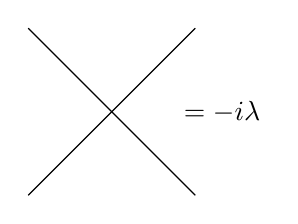
\begin{tikzpicture}[scale=0.7]
            \begin{feynman}
                \vertex (o);
                \vertex [below right =of o] (f2);
                \vertex [below left =of o] (i2);                
                \vertex [above right =of o] (f1);
                \vertex [above left =of o] (i1);
                \diagram*{
                    (i1) --  (o) -- (f1);
                    (i2) -- (o) -- (f2);
                };
            \end{feynman}
            \node at (2,0) {\(=-i\lambda\)};
        \end{tikzpicture}
    \end{figure}
    where \(-i\lambda\) is the value associated with the vertex. Notice that we are not putting the \(4!\), since the symmetry of the diagram already takes care of it.\\

    In addition, we are supposed to associate momenta with each leg of a vertex, and impose energy momentum conservation, i.e.     
    \begin{figure}[h]
        \centering
        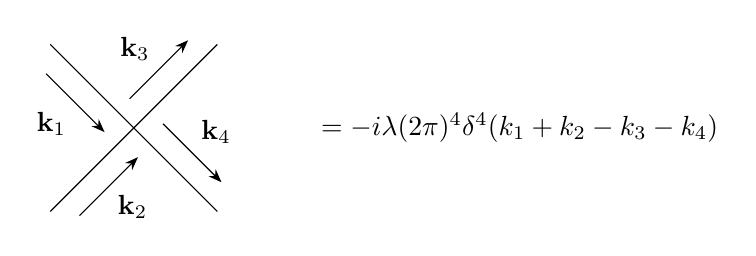
\begin{tikzpicture}[scale=0.7]
            \begin{feynman}
                \vertex (o);
                \vertex [below right =of o] (f2);
                \vertex [below left =of o] (i2);                
                \vertex [above right =of o] (f1);
                \vertex [above left =of o] (i1);
                \diagram*{
                    (i1) -- [ momentum'=$\textbf{k}_1$] (o) --[ momentum=$\textbf{k}_3$] (f1);
                    (i2) -- [ momentum'=$\textbf{k}_2$](o) --[ momentum=$\textbf{k}_4$] (f2);
                };
            \end{feynman}
            \node at (7,0) {\(=-i\lambda(2\pi)^4\delta^4(k_1 + k_2 - k_3 - k_4)\)};
        \end{tikzpicture}
    \end{figure}

    What about the \(\phi\psi\psi^\dagger\) model? Now there are two kinds of particles, and therefore we need to come up with a notation. Let us call the dotted line \(\phi\), line with arrow pointing towards the vertex \(\psi\) and the line with arrow pointing away \(\psi^\dagger\). Therefore, the vertex is 
    \begin{figure}[h]
        \centering
        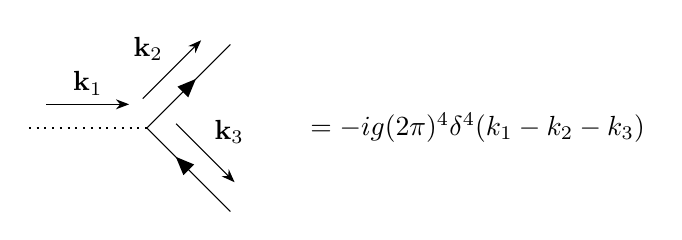
\begin{tikzpicture}[scale=0.7]
            \begin{feynman}
                \vertex (o);
                \vertex [left =of o] (i);                
                \vertex [above right =of o] (f1);
                \vertex [below right =of o] (f2);
                \diagram*{
                    (i) --[ghost, momentum=$\textbf{k}_1$] (o);
                    (o) -- [fermion, momentum=$\textbf{k}_2$] (f1);
                    (o) -- [anti fermion, momentum=$\textbf{k}_3$] (f2);
                };
            \end{feynman}
            \node at (6,0) {\(=-ig(2\pi)^4\delta^4(k_1 - k_2 - k_3)\)};
        \end{tikzpicture}
    \end{figure}




\end{document}
